\documentclass[10pt,a4paper,oneside]{report}

% =====================================================================
% PACKAGES
% =====================================================================
\usepackage[utf8]{inputenc}
\usepackage[T1]{fontenc}
\usepackage[english]{babel}
\usepackage{geometry}
\usepackage{graphicx}
\usepackage{caption}
\usepackage{subcaption}
\usepackage{booktabs}
\usepackage{longtable}
\usepackage{array}
\usepackage{multirow}
\usepackage{makecell}
\usepackage{float}
\usepackage{amsmath}
\usepackage{amssymb}
\usepackage{amsfonts}
\usepackage{mathtools}
\usepackage{algorithm}
\usepackage{algpseudocode}
\usepackage{tikz}
\usepackage{pgfplots}
\usepackage{pgfplotstable}
\usepackage{listings}
\usepackage{xcolor}
\usepackage{hyperref}
\usepackage{cleveref}
\usepackage{acronym}
\usepackage{enumitem}
\usepackage{setspace}
\usepackage{titlesec}
\usepackage{fancyhdr}
\usepackage{lastpage}
\usepackage{csquotes}
\usepackage{textcomp}
\usepackage{newunicodechar}
\usepackage{etoolbox}

% =====================================================================
% UNICODE CHARACTER SUPPORT
% =====================================================================
\newunicodechar{✅}{\textbullet\ }
\newunicodechar{⚠}{\textasteriskcentered\ }
\newunicodechar{⚠️}{\textasteriskcentered\ }
\newunicodechar{✓}{\textbullet}
\newunicodechar{α}{\ensuremath{\alpha}}
\newunicodechar{≥}{\ensuremath{\geq}}
\newunicodechar{≤}{\ensuremath{\leq}}
\newunicodechar{→}{\ensuremath{\rightarrow}}
\newunicodechar{×}{\ensuremath{\times}}
\newunicodechar{–}{\textendash}
\newunicodechar{—}{\textemdash}
\newunicodechar{·}{\textperiodcentered}
\newunicodechar{♯}{\#}
\newunicodechar{♥}{\textheartsuit}
\newunicodechar{★}{\textasteriskcentered}

% =====================================================================
% GEOMETRY & LAYOUT
% =====================================================================
\usepackage{geometry}
\geometry{
    a4paper,
    left=25mm,
    right=25mm,
    top=25mm,
    bottom=25mm,
    headheight=14pt,
    headsep=8mm,
    footskip=12mm
}

\usepackage{setspace}
\setstretch{1.15}
\setlength{\parindent}{1em}
\setlength{\parskip}{0.3em}

% =====================================================================
% COLORS
% =====================================================================
\definecolor{trackvisionblue}{RGB}{0, 100, 170}
\definecolor{trackvisiondark}{RGB}{30, 30, 30}
\definecolor{trackvisiongray}{RGB}{80, 80, 80}
\definecolor{codebg}{RGB}{248, 248, 248}
\definecolor{keyword}{RGB}{0, 0, 140}
\definecolor{comment}{RGB}{0, 110, 0}
\definecolor{string}{RGB}{150, 0, 0}
\definecolor{number}{RGB}{0, 0, 180}
\definecolor{rowcolor}{RGB}{240, 245, 250}

% =====================================================================
% TITLE FORMATTING - SIMPLE, NO NESTED TITLES
% =====================================================================
\titleformat{\chapter}[display]
    {\normalfont\Large\bfseries\color{trackvisiondark}}
    {\MakeUppercase{\chaptertitlename}\ \thechapter}
    {10pt}
    {\titlerule[1pt]\vspace{6pt}\centering}
    [\vspace{4pt}\titlerule[0.5pt]]

\titleformat{\section}
    {\normalfont\large\bfseries\color{trackvisiondark}}
    {\thesection}{0.6em}{}

\titleformat{\subsection}
    {\normalfont\normalsize\bfseries\color{trackvisionblue}}
    {\thesubsection}{0.6em}{}

\titleformat{\subsubsection}
    {\normalfont\small\bfseries\color{trackvisionblue}}
    {\thesubsubsection}{0.6em}{}

% =====================================================================
% LISTINGS CONFIGURATION - WITH JAVASCRIPT/TYPESCRIPT SUPPORT
% =====================================================================
\usepackage{listings}
\lstdefinelanguage{TypeScript}{
    morekeywords={abstract, as, async, await, boolean, break, case, catch, class, const, continue, debugger, declare, default, delete, do, else, enum, export, extends, false, finally, for, from, function, get, if, implements, import, in, instanceof, interface, let, module, namespace, never, new, null, number, of, package, private, protected, public, readonly, return, set, static, string, super, switch, symbol, this, throw, true, try, type, typeof, undefined, var, void, while, with, yield, async, await, of, type, keyof, infer, unknown, any, never, bigint, constructor, static, get, set, infer, keyof, declare, declare, type, interface, enum, implements, extends, public, private, protected, readonly, abstract, override, static, async, await},
    sensitive=true,
    morecomment=[l]{//},
    morecomment=[s]{/*}{*/},
    morestring=[b]",
    morestring=[b]',
    morestring=[b]`,
}
\lstdefinestyle{typescript}{
    language=TypeScript,
    backgroundcolor=\color{codebg},
    basicstyle=\ttfamily\scriptsize,
    keywordstyle=\color{keyword}\bfseries,
    commentstyle=\color{comment}\itshape,
    stringstyle=\color{string},
    numberstyle=\color{number}\tiny,
    numbers=left,
    numbersep=3pt,
    stepnumber=1,
    numberfirstline=true,
    frame=single,
    framesep=3pt,
    rulecolor=\color{trackvisionblue!20},
    breaklines=true,
    breakatwhitespace=false,
    tabsize=2,
    showspaces=false,
    showstringspaces=false,
    columns=fullflexible,
    keepspaces=true,
    linewidth=\linewidth,
    xleftmargin=0pt,
    xrightmargin=0pt,
}
\lstdefinestyle{pseudocode}{
    basicstyle=\ttfamily\scriptsize,
    keywordstyle=\color{keyword}\bfseries,
    commentstyle=\color{comment}\itshape,
    numbers=left,
    numbersep=3pt,
    frame=single,
    framesep=3pt,
    rulecolor=\color{trackvisionblue!20},
    breaklines=true,
    tabsize=2,
    linewidth=\linewidth,
}

% =====================================================================
% TIKZ/PGFPLOTS CONFIGURATION
% =====================================================================
\usepackage{pgfplots}
\pgfplotsset{compat=1.18}
\usetikzlibrary{
    shapes.geometric,
    shapes.arrows,
    arrows.meta,
    positioning,
    fit,
    backgrounds,
    calc,
    decorations.pathreplacing,
    calligraphy,
    shadows,
    matrix,
    chains,
    arrows
}

% =====================================================================
% HYPERREF CONFIGURATION
% =====================================================================
\usepackage{hyperref}
\hypersetup{
    colorlinks=true,
    linkcolor=trackvisionblue,
    filecolor=trackvisionblue,
    urlcolor=trackvisionblue,
    citecolor=trackvisionblue,
    pdfauthor={TrackVision Team},
    pdfsubject={Unit 2 Computer Vision Mini Project - Multiple Object Tracking in Video},
    pdfkeywords={Computer Vision, Multiple Object Tracking, ByteTrack, YOLO, Kalman Filter, ONNX Runtime Web},
    pdftitle={TrackVision: Real-time Client-Side Multiple Object Tracking},
    pdfproducer={LaTeX with pdfTeX},
    bookmarksopen=true,
    bookmarksdepth=3
}

% =====================================================================
% FANCY HEADERS
% =====================================================================
\usepackage{fancyhdr}
\pagestyle{fancy}
\fancyhf{}
\fancyhead[L]{\nouppercase{\leftmark}}
\fancyhead[R]{\thepage}
\fancyfoot[C]{}
\renewcommand{\headrulewidth}{0.4pt}
\renewcommand{\footrulewidth}{0pt}

\fancypagestyle{plain}{
    \fancyhf{}
    \fancyfoot[C]{\thepage}
    \renewcommand{\headrulewidth}{0pt}
}

% =====================================================================
% CUSTOM COMMANDS
% =====================================================================
\newcommand{\todo}[1]{\textcolor{red}{[TODO: #1]}}
\newcommand{\placeholder}[1]{\textcolor{red}{[INSERT SCREENSHOT: #1]}}
\newcommand{\trackvision}{\textsc{TrackVision}}
\newcommand{\bytetrack}{\textsc{ByteTrack++}}
\newcommand{\yolo}{\textsc{YOLOv8n}}
\newcommand{\yoloworld}{\textsc{YOLO-World}}
\newcommand{\clip}{\textsc{CLIP} ViT-B/32}
\newcommand{\osnet}{\textsc{OSNet} x1.0}
\newcommand{\onnxweb}{\textsc{ONNX} Runtime Web}
\newcommand{\webgpu}{WebGPU}
\newcommand{\wasm}{WASM}
\newcommand{\webnn}{WebNN}
\newcommand{\webgl}{WebGL}
\newcommand{\e}{\ensuremath{\epsilon}}
\newcommand{\R}{\mathbb{R}}

% =====================================================================
% ACRONYMS
% =====================================================================
\usepackage{acronym}
\acrodef{MOT}[MOT]{Multiple Object Tracking}
\acrodef{SOT}[SOT]{Single Object Tracking}
\acrodef{YOLO}[YOLO]{You Only Look Once}
\acrodef{CNN}[CNN]{Convolutional Neural Network}
\acrodef{RNN}[RNN]{Recurrent Neural Network}
\acrodef{KF}[KF]{Kalman Filter}
\acrodef{EKF}[EKF]{Extended Kalman Filter}
\acrodef{UKF}[UKF]{Unscented Kalman Filter}
\acrodef{IOU}[IoU]{Intersection over Union}
\acrodef{NMS}[NMS]{Non-Maximum Suppression}
\acrodef{ReID}[ReID]{Re-Identification}
\acrodef{CLIP}[CLIP]{Contrastive Language-Image Pre-training}
\acrodef{BPE}[BPE]{Byte Pair Encoding}
\acrodef{API}[API]{Application Programming Interface}
\acrodef{UI}[UI]{User Interface}
\acrodef{FPS}[FPS]{Frames Per Second}
\acrodef{GPU}[GPU]{Graphics Processing Unit}
\acrodef{CPU}[CPU]{Central Processing Unit}
\acrodef{RAM}[RAM]{Random Access Memory}
\acrodef{SSD}[SSD]{Solid State Drive}
\acrodef{HTTP}[HTTP]{Hypertext Transfer Protocol}
\acrodef{HTTPS}[HTTPS]{Hypertext Transfer Protocol Secure}
\acrodef{JSON}[JSON]{JavaScript Object Notation}
\acrodef{HTML}[HTML]{Hypertext Markup Language}
\acrodef{CSS}[CSS]{Cascading Style Sheets}
\acrodef{DOM}[DOM]{Document Object Model}
\acrodef{WASM}[WASM]{WebAssembly}
\acrodef{SIMD}[SIMD]{Single Instruction Multiple Data}
\acrodef{EP}[EP]{Execution Provider}
\acrodef{PWA}[PWA]{Progressive Web App}
\acrodef{CI}[CI]{Continuous Integration}
\acrodef{CD}[CD]{Continuous Deployment}

% =====================================================================
% TABLES - PROFESSIONAL STYLING
% =====================================================================
\newcommand{\tablerowcolors}{\rowcolors{2}{rowcolor}{white}}

% =====================================================================
% DOCUMENT START
% =====================================================================
\begin{document}

% =====================================================================
% FRONT MATTER
% =====================================================================
% =====================================================================
% FRONT MATTER
% =====================================================================

% ---------------------------------------------------------------------
% COVER PAGE
% ---------------------------------------------------------------------
\begin{titlepage}
    \centering
    \vspace*{2cm}
    
    {\Huge \bfseries \color{trackvisiondark} TrackVision}\\[0.5cm]
    {\LARGE \color{trackvisionblue} Real-time Client-Side Multiple Object Tracking in Video}\\[2cm]
    
    % 
\includegraphics[width=0.4\textwidth]{figures/01-landing-page.png}\\[2cm]
    
    {\large \bfseries Unit 2 Computer Vision Mini Project}\\[1cm]
    
    {\large Submitted in partial fulfillment of the requirements for the degree of}\\[0.5cm]
    {\large Bachelor of Technology in Computer Science and Engineering}\\[2cm]
    
    \begin{tabular}{ll}
        \bfseries Student: & [Student Name] \\
        \bfseries Roll Number: & [Roll Number] \\
        \bfseries Branch: & Computer Science and Engineering \\
        \bfseries Semester: & [Semester] \\
        \bfseries Academic Year: & 2025--2026 \\
        \bfseries Submission Date: & 12 September 2026 \\
        \bfseries Guide: & [Guide Name] \\
        \bfseries Department: & Department of Computer Science and Engineering \\
        \bfseries Institute: & [Institute Name] \\
    \end{tabular}
    
    \vfill
    
    {\color{trackvisiongray} \textit{TrackVision -- Precision Object Intelligence}}
    
    \vspace{1cm}
\end{titlepage}

% ---------------------------------------------------------------------
% CERTIFICATE
% ---------------------------------------------------------------------
\chapter*{Certificate}
\thispagestyle{plain}
\addcontentsline{toc}{chapter}{Certificate}

\vspace{2cm}

\noindent This is to certify that the project report entitled \textbf{``TrackVision: Real-time Client-Side Multiple Object Tracking in Video''} submitted by \textbf{[Student Name]} (Roll No: [Roll Number]) in partial fulfillment of the requirements for the award of the degree of \textbf{Bachelor of Technology in Computer Science and Engineering} is a bonafide record of work carried out by him/her under my supervision and guidance.

\vspace{1.5cm}

\noindent The project represents the student's own work and has not been submitted elsewhere for any other degree or diploma.

\vspace{2cm}

\begin{tabular}{p{7cm} p{7cm}}
    \hrulefill & \hrulefill \\
    \textbf{[Guide Name]} & \textbf{[Head of Department]} \\
    Project Guide & Department of CSE \\
    Department of CSE & [Institute Name] \\
    [Institute Name] & \\
    Date: \today & Date: \today \\
\end{tabular}

\newpage

% ---------------------------------------------------------------------
% DECLARATION
% ---------------------------------------------------------------------
\chapter*{Declaration}
\thispagestyle{plain}
\addcontentsline{toc}{chapter}{Declaration}

\vspace{2cm}

\noindent I, \textbf{[Student Name]}, Roll Number \textbf{[Roll Number]}, student of \textbf{Bachelor of Technology in Computer Science and Engineering}, hereby declare that the project report entitled \textbf{``TrackVision: Real-time Client-Side Multiple Object Tracking in Video''} is an original work carried out by me under the guidance of \textbf{[Guide Name]}, Department of Computer Science and Engineering, \textbf{[Institute Name]}.

\vspace{1cm}

\noindent This work has not been submitted to any other university or institution for the award of any degree or diploma. All sources of information used in this report have been duly acknowledged.

\vspace{2cm}

\noindent \hrulefill \\
\textbf{[Student Name]} \\
Roll No: [Roll Number] \\
Date: \today \\
Place: [City]

\newpage

% ---------------------------------------------------------------------
% ABSTRACT
% ---------------------------------------------------------------------
\chapter*{Abstract}
\thispagestyle{plain}
\addcontentsline{toc}{chapter}{Abstract}

\vspace{1cm}

\noindent \textbf{Multiple Object Tracking (MOT)} is a fundamental computer vision task that extends object detection by maintaining consistent object identities across consecutive video frames. Traditional MOT systems typically operate on powerful servers with GPU acceleration, requiring video uploads and introducing latency, privacy concerns, and bandwidth costs.

\vspace{0.5cm}

\noindent This project presents \trackvision, a fully client-side MOT system that runs entirely within a web browser using \onnxweb for hardware-accelerated inference. The system implements a custom \bytetrack algorithm with a full 6x6 covariance Kalman filter, Hungarian data association, and optional OSNet x1.0 appearance-based re-identification. Two detection modes are supported: a fast path using YOLOv8n (COCO-80 classes, 12.8 MB) and an open-vocabulary path using YOLO-World with CLIP ViT-B/32 text embeddings computed in-browser.

\vspace{0.5cm}

\noindent The architecture employs four Web Workers (YOLO detection, YOLO-World, ReID, Tracker) communicating via a typed message protocol, with the main thread handling class-aware NMS, visualization, and state management via Zustand. Video input is captured via \texttt{OffscreenCanvas} at 640x640 letterboxed resolution. The system achieves sub-millisecond JavaScript-side tracking overhead (0.31--1.04 ms/frame at 5--20 detections) and provides real-time telemetry (FPS, latency breakdown, execution provider).

\vspace{0.5cm}

\noindent \textbf{Key contributions:} (1) A production-grade client-side MOT pipeline with zero server dependencies, (2) Dual detection modes with in-browser CLIP text encoding, (3) Custom TypeScript ByteTrack++ with full covariance Kalman filtering and appearance fusion, (4) Comprehensive UI with Ghost/Follow/Replay modes, 5-minute history, and analytics, (5) 49 unit tests validating core algorithms, (6) Static deployment with COOP/COEP headers for WebGPU/SharedArrayBuffer support.

\vspace{0.5cm}

\noindent \textbf{Limitations:} No formal benchmark dataset is used; standardized MOT metrics (MOTA, IDF1, HOTA) are not computed. Evaluation consists of implementation-level unit tests, microbenchmarks, and qualitative observation. Future work includes MOTChallenge evaluation integration and video file upload support.

\vspace{1cm}

\noindent \textbf{Keywords:} Multiple Object Tracking, ByteTrack, YOLOv8, YOLO-World, Kalman Filter, Hungarian Algorithm, OSNet, CLIP, ONNX Runtime Web, WebGPU, Client-Side Inference

\newpage

% ---------------------------------------------------------------------
% ACKNOWLEDGEMENT
% ---------------------------------------------------------------------
\chapter*{Acknowledgement}
\thispagestyle{plain}
\addcontentsline{toc}{chapter}{Acknowledgement}

\vspace{2cm}

\noindent I would like to express my sincere gratitude to all those who have contributed to the successful completion of this project.

\vspace{1cm}

\noindent First and foremost, I am deeply grateful to my project guide \textbf{[Guide Name]} for their invaluable guidance, constant encouragement, and constructive feedback throughout the project. Their expertise and insights were instrumental in shaping the technical direction of this work.

\vspace{1cm}

\noindent I extend my thanks to \textbf{[Head of Department]}, Head of the Department of Computer Science and Engineering, for providing the necessary infrastructure and support.

\vspace{1cm}

\noindent I am thankful to the faculty members of the Department of Computer Science and Engineering for their academic guidance and for creating an environment conducive to learning and innovation.

\vspace{1cm}

\noindent This project stands on the shoulders of giants in the computer vision and open-source communities. I acknowledge the authors and maintainers of:

\vspace{0.5cm}

\begin{itemize}
    \item \textbf{ByteTrack} -- YOLOX/ByteTrack \cite{zhang2021bytetrack}
    \item \textbf{YOLOv8} -- Ultralytics \cite{jocher2023ultralytics}
    \item \textbf{YOLO-World} -- AILab-CVC/YOLO-World \cite{cheng2024yoloworld}
    \item \textbf{OSNet} -- Kaiyang Zhou \cite{zhou2019osnet}
    \item \textbf{CLIP} -- OpenAI \cite{radford2021clip}
    \item \textbf{ONNX Runtime Web} -- Microsoft \cite{ortweb}
    \item \textbf{React, Vite, Tailwind CSS, Zustand, Recharts} -- Respective open-source communities
\end{itemize}

\vspace{1cm}

\noindent Special thanks to the developers of \texttt{onnxruntime-web}, \texttt{wkentaro/yolo-world-onnx}, and \texttt{Xenova/transformers.js} for providing the ONNX models and tokenizer assets that make in-browser open-vocabulary detection possible.

\vspace{1cm}

\noindent Finally, I thank my peers and family for their unwavering support and patience during the long hours of development and documentation.

\vspace{2cm}

\noindent \hrulefill \\
\textbf{[Student Name]} \\
Roll No: [Roll Number]

\newpage

% =====================================================================
% TABLE OF CONTENTS
% =====================================================================
\tableofcontents
\newpage
\listoffigures
\newpage
\listoftables
\newpage

% =====================================================================
% MAIN CHAPTERS
% =====================================================================
% =====================================================================
% CHAPTER 1: AIM
% =====================================================================
\chapter{Aim}
\label{ch:aim}

The aim of this project is to \textbf{design, implement, and evaluate a real-time, fully client-side multiple object tracking system capable of detecting, associating, and maintaining persistent object identities across consecutive video frames directly within a web browser}, without requiring any server-side computation or video upload.

\vspace{0.5cm}

\noindent The specific objectives are:

\begin{enumerate}
    \item \textbf{Client-side inference pipeline:} Implement a complete MOT pipeline (detection $\to$ NMS $\to$ ReID $\to$ tracking $\to$ visualization) using \onnxweb with hardware acceleration (WebNN $\to$ WebGPU $\to$ WebGL $\to$ WASM cascade), ensuring zero data leaves the user's device.
    
    \item \textbf{Dual detection modes:} Support both a fast, fixed-vocabulary mode (YOLOv8n, 80 COCO classes) and an open-vocabulary mode (YOLO-World + CLIP ViT-B/32 text embeddings) with in-browser tokenization and text encoding.
    
    \item \textbf{Custom ByteTrack++ tracker:} Implement a tracking-by-detection algorithm with:
    \begin{itemize}
        \item Full 6x6 covariance Kalman filter (constant acceleration model)
        \item Hungarian algorithm for optimal data association
        \item Track lifecycle management (TENTATIVE $\to$ CONFIRMED $\to$ LOST $\to$ REMOVED)
        \item Appearance-based re-identification via OSNet x1.0 (512-dim embeddings)
        \item EMA appearance fusion ($\alpha=0.3$) and track merging for split-identity recovery
        \item EMA bounding-box smoothing ($\alpha=0.7$) and occlusion interpolation (up to 5 frames)
    \end{itemize}
    
    \item \textbf{Browser-native video acquisition:} Capture live camera feed via \texttt{getUserMedia()} and process frames using \texttt{OffscreenCanvas} at 640x640 letterboxed resolution with zero-copy buffer transfer to workers.
    
    \item \textbf{Real-time telemetry and history:} Provide per-frame latency breakdown (preprocess, inference, postprocess, tracking, render), FPS monitoring, 5-minute rolling history with frame-perfect replay, and persistent track metadata (trajectories, distance, speed, bearing).
    
    \item \textbf{Comprehensive UI/UX:} Implement a responsive Command Center with Ghost mode (trajectory trails), Follow mode (target lock), Time Machine (history scrubber), Scene Map (2D density), Analytics (class distribution, volume charts), and Command Palette.
    
    \item \textbf{Validation and deployment:} Achieve 49 passing unit tests covering Kalman filtering, Hungarian matching, ByteTrack lifecycle, appearance fusion, NMS, and store history; produce a production build deployable to static hosts (Netlify, Vercel, Cloudflare Pages) with required COOP/COEP headers.
\end{enumerate}

\vspace{0.5cm}

\noindent The system is evaluated through implementation-level tests, runtime microbenchmarks, telemetry observation, and qualitative tracking behavior assessment. Standardized MOT benchmark metrics (MOTA, IDF1, HOTA) are \textbf{not computed} in the current implementation due to the absence of a formal annotated dataset; this is documented as a limitation and future work direction.

\vspace{0.5cm}

\noindent \textbf{Scope:} The project demonstrates that a complete, production-quality MOT system can run entirely in-browser using modern web APIs and ONNX Runtime Web, achieving real-time performance on consumer hardware while preserving user privacy and eliminating server costs.
% =====================================================================
% CHAPTER 2: INTRODUCTION
% =====================================================================
\chapter{Introduction}
\label{ch:introduction}

\section{Computer Vision}
\label{sec:cv}

Computer Vision (CV) is an interdisciplinary field that enables computers to derive meaningful understanding from digital images or videos. It seeks to automate tasks that the human visual system performs effortlessly: identifying objects, recognizing scenes, detecting motion, and understanding spatial relationships. Over the past decade, deep learning — particularly Convolutional Neural Networks (CNNs) — has revolutionized CV, achieving superhuman performance on benchmarks such as ImageNet classification \cite{russakovsky2015imagenet}, COCO object detection \cite{lin2014coco}, and KITTI autonomous driving \cite{geiger2012kitti}.

\section{Video Analysis}
\label{sec:video-analysis}

Video analysis extends CV from static images to temporal sequences. A video is a sequence of frames, typically captured at 24--60 FPS, where each frame is correlated with its neighbors. The temporal dimension introduces both challenges (motion blur, occlusion, appearance change) and opportunities (motion cues, track continuity, action recognition). Core video analysis tasks include action recognition, video object segmentation, and multiple object tracking.

\section{Object Detection}
\label{sec:object-detection}

Object detection answers the question: \textit{``What objects are present in this frame, and where?''} Given an image, a detector outputs a set of bounding boxes with class labels and confidence scores. Modern detectors fall into two families:

\begin{itemize}
    \item \textbf{Two-stage detectors} (R-CNN \cite{girshick2014rcnn}, Faster R-CNN \cite{ren2015faster}): Region proposal $\to$ classification/regression. High accuracy, slower.
    \item \textbf{Single-stage detectors} (YOLO \cite{redmon2016yolo}, SSD \cite{liu2016ssd}, RetinaNet \cite{lin2017retinanet}): Direct prediction from dense grid. Faster, suitable for real-time.
\end{itemize}

YOLO (You Only Look Once) pioneered real-time detection by framing it as a single regression problem. YOLOv8 \cite{jocher2023ultralytics} represents the current state-of-the-art in the YOLO lineage, offering improved accuracy-speed tradeoffs and a unified architecture for detection, segmentation, and pose estimation.

\section{Object Tracking}
\label{sec:object-tracking}

Object tracking answers: \textit{``Where did the object detected in the previous frame go?''} Unlike detection (per-frame, independent), tracking maintains \textit{identity} across time.

\subsection{Single Object Tracking (SOT)}
\label{sec:sot}
SOT initializes with a ground-truth bounding box in frame 1 and predicts the target's location in subsequent frames. Approaches include correlation filters (MOSSE \cite{bolme2010mosse}, CSRT \cite{lukezic2017csrt}) and Siamese networks (SiamFC \cite{bertinetto2016siamfc}, SiamRPN \cite{li2018siamrpn}). SOT assumes the target is always present and does not handle multiple objects or identity assignment.

\subsection{Multiple Object Tracking (MOT)}
\label{sec:mot}
MOT extends SOT to \textit{multiple simultaneous objects} with \textit{unknown and variable count}. The core challenge is \textbf{data association}: given detections in frame $t$ and tracks from frame $t-1$, which detection belongs to which track? MOT systems typically follow the \textbf{tracking-by-detection} paradigm:

\begin{enumerate}
    \item Detect objects in each frame independently.
    \item Associate detections across frames to form trajectories.
    \item Manage track lifecycle (initialization, confirmation, loss, deletion).
\end{enumerate}

The distinction is fundamental:
\begin{quote}
\textbf{Object detection} answers: ``What objects are present in \textit{this} frame?'' \\
\textbf{Multiple object tracking} answers: ``Which detected object corresponds to \textit{which previously observed object}?''
\end{quote}

\section{Problem Statement}
\label{sec:problem}

Despite advances in MOT algorithms, \textbf{deployment remains a barrier}. Most MOT systems:
\begin{itemize}
    \item Require server-grade GPUs (CUDA, cuDNN, TensorRT).
    \item Necessitate video upload (bandwidth, latency, privacy).
    \item Depend on complex Python/C++ stacks (PyTorch, TensorFlow, OpenCV).
    \item Lack cross-platform accessibility (Windows/Linux/macOS, mobile).
\end{itemize}

There is a need for a \textbf{zero-installation, privacy-preserving, cross-platform MOT system} that runs entirely on the client device using only standard web APIs.

\section{Motivation}
\label{sec:motivation}

\begin{enumerate}
    \item \textbf{Privacy:} Video data never leaves the device. Critical for surveillance, healthcare, retail analytics.
    \item \textbf{Latency:} No network round-trip. Enables real-time interactive applications (AR, robotics, gaming).
    \item \textbf{Accessibility:} Runs in any modern browser (Chrome, Edge, Firefox, Safari) on desktop or mobile.
    \item \textbf{Cost:} Zero server infrastructure. Scales to millions of users with static hosting.
    \item \textbf{WebGPU:} Emerging standard exposes GPU compute to the web, enabling near-native inference speed.
\end{enumerate}

\section{Objectives}
\label{sec:objectives}

\begin{enumerate}
    \item Implement a client-side MOT pipeline with YOLOv8n (fast) and YOLO-World + CLIP (open-vocabulary) detection.
    \item Develop a custom ByteTrack++ tracker in TypeScript with full covariance Kalman filtering and Hungarian association.
    \item Integrate OSNet x1.0 ReID for appearance-based occlusion recovery.
    \item Build a responsive web UI with real-time telemetry, history replay, and multiple visualization modes.
    \item Validate core algorithms with 49 unit tests; measure pipeline performance.
    \item Deploy as a static PWA with WebGPU acceleration and HTTPS support for mobile camera access.
\end{enumerate}

\section{Scope}
\label{sec:scope}

\begin{itemize}
    \item \textbf{In scope:} Real-time browser MOT, dual detection modes, custom tracker, ReID, UI/UX, deployment.
    \item \textbf{Out of scope:} Standardized MOT benchmark evaluation (MOTA/IDF1/HOTA), video file upload (camera only), server-side components, 3D tracking, pose estimation, action recognition.
\end{itemize}

\section{Project Contribution}
\label{sec:contribution}

This project contributes a \textbf{complete, production-grade, client-side MOT system} implemented in TypeScript/React that demonstrates:
\begin{itemize}
    \item The feasibility of running YOLO + ByteTrack + Kalman + ReID entirely in-browser via ONNX Runtime Web.
    \item A novel open-vocabulary detection path using in-browser CLIP text encoding (no external embedding service).
    \item A clean, typed Web Worker architecture with typed message protocols.
    \item Comprehensive UI/UX for MOT visualization and analysis.
    \item Open-source deployment model (static hosting, Docker, MIT license).
\end{itemize}
% =====================================================================
% CHAPTER 3: LITERATURE REVIEW
% =====================================================================
\chapter{Literature Review}
\label{ch:literature}

\section{Traditional Object Tracking}
\label{sec:traditional-tracking}

Before deep learning, tracking relied on hand-crafted features and probabilistic filters. The \textbf{Kalman Filter} \cite{kalman1960new} provides optimal state estimation for linear Gaussian systems. For visual tracking, the \textbf{Mean Shift} algorithm \cite{comaniciu2002meanshift} iteratively seeks the mode of a target's color histogram. \textbf{Optical flow} methods (Lucas-Kanade \cite{lucas1981iterative}, Farnebäck \cite{farneback2003twoframe}) estimate dense or sparse motion fields between frames. These approaches are computationally efficient but struggle with appearance changes, occlusion, and long-term identity maintenance.

\section{Tracking-by-Detection Paradigm}
\label{sec:tracking-by-detection}

Modern MOT predominantly follows the \textbf{tracking-by-detection} paradigm \cite{bewley2016sort}: an independent object detector runs per frame, and a tracker associates detections across time. This decouples detection quality from tracking logic and allows plug-and-play detector upgrades.

\section{SORT and Deep SORT}
\label{sec:sort-deepsort}

\textbf{SORT (Simple Online and Realtime Tracking)} \cite{bewley2016sort} combines a Kalman filter (constant velocity model) with Hungarian assignment based on IoU. It is fast and effective for low occlusion but lacks appearance information, leading to ID switches when objects cross or are occluded.

\textbf{Deep SORT} \cite{wojke2017deepsort} extends SORT by integrating a deep appearance descriptor (a CNN trained on person re-identification). The association cost fuses IoU and cosine distance between embeddings. This significantly reduces ID switches but increases computational cost.

\section{ByteTrack}
\label{sec:bytetrack}

\textbf{ByteTrack} \cite{zhang2021bytetrack} observes that low-confidence detections (often discarded by SORT/Deep SORT) contain valuable information for tracking occluded or small objects. It introduces a two-stage association:
\begin{enumerate}
    \item High-confidence detections ($\ge$ trackThresh) matched with all tracks.
    \item Low-confidence detections matched only with unmatched tracks.
\end{enumerate}
This simple modification achieves state-of-the-art MOTA on MOT17 without appearance features. ByteTrack also uses a more robust Kalman filter and track lifecycle management.

\section{BoT-SORT and StrongSORT}
\label{sec:botsort-strongsort}

\textbf{BoT-SORT} \cite{aharon2022botsort} improves ByteTrack with camera motion compensation (CMC) and a more sophisticated appearance model. \textbf{StrongSORT} \cite{du2023strongsort} combines BoT-SORT's improvements with an enhanced ReID model (OSNet-AIN) and adaptive appearance weighting. Both achieve higher MOTA/IDF1 at increased complexity.

\section{YOLO Family}
\label{sec:yolo-family}

\begin{itemize}
    \item \textbf{YOLOv1--v3} \cite{redmon2016yolo,redmon2017yolo9000,redmon2018yolov3}: Progressive improvements in speed/accuracy.
    \item \textbf{YOLOv4} \cite{bochkovskiy2020yolov4}: CSPDarknet53 backbone, PANet neck, Mish activation.
    \item \textbf{YOLOv5} \cite{jocher2021yolov5}: PyTorch reimplementation, widely adopted, export-friendly.
    \item \textbf{YOLOv8} \cite{jocher2023ultralytics}: Unified architecture for detection/segmentation/pose; anchor-free; improved head.
\end{itemize}

YOLOv8n (nano) is the smallest variant ($\sim$3.2M parameters, 12.8 MB ONNX), suitable for real-time edge/browser deployment.

\section{YOLO-World: Open-Vocabulary Detection}
\label{sec:yoloworld}

Traditional detectors are limited to fixed training vocabularies (e.g., COCO-80). \textbf{YOLO-World} \cite{cheng2024yoloworld} enables \textit{open-vocabulary} detection by conditioning on text embeddings. It uses a \textbf{RepVL-PAN} neck that fuses visual features with CLIP \cite{radford2021clip} text embeddings. At inference, user-supplied concepts are encoded by CLIP's text encoder and fed as \texttt{text\_features} to the detector. This enables zero-shot detection of arbitrary categories without retraining.

\section{CLIP: Contrastive Language-Image Pre-training}
\label{sec:clip}

\textbf{CLIP} \cite{radford2021clip} learns joint image-text representations by contrastive pre-training on 400M image-text pairs. The text encoder (Transformer) maps tokenized captions to 512-dim embeddings; the image encoder (ViT or ResNet) maps images to the same space. Zero-shot classification uses cosine similarity between image and text embeddings. CLIP ViT-B/32 uses a Vision Transformer (ViT-B/32) image encoder and a 12-layer Transformer text encoder.

\section{OSNet: Omni-Scale Network for ReID}
\label{sec:osnet}

\textbf{OSNet} \cite{zhou2019osnet} is a lightweight CNN for person re-identification. Its Omni-Scale residual block captures features at multiple spatial scales simultaneously. OSNet x1.0 ($\sim$2.2M parameters) produces 512-dim embeddings and achieves strong accuracy on Market-1501 / DukeMTMC-reID. The ONNX export (Axelera mirror) expects 256x128 crops with ImageNet normalization.

\section{Kalman Filter in Visual Tracking}
\label{sec:kf-tracking}

The Kalman filter \cite{kalman1960new} is the workhorse of MOT state estimation. For 2D bounding box tracking, the state vector typically includes position, velocity, and optionally size:
\[
\mathbf{x} = [x, y, v_x, v_y, w, h]^T
\]
The constant velocity model assumes $x_{t+1} = x_t + v_x \Delta t$. Process noise models acceleration uncertainty; measurement noise models detection jitter. Full covariance (6x6) propagation captures correlations between state variables (e.g., position-velocity coupling).

\section{Hungarian Algorithm for Data Association}
\label{sec:hungarian}

The assignment problem (minimize total cost of matching tracks to detections) is solved optimally in $O(n^3)$ by the \textbf{Hungarian algorithm} (Kuhn-Munkres) \cite{kuhn1955hungarian,munkres1957algorithms}. The cost matrix typically uses $1 - \text{IoU}$ or a fusion of IoU, appearance distance, and class consistency. Gating (thresholding impossible assignments) reduces the problem size.

\section{Browser-Based Inference}
\label{sec:browser-inference}

\textbf{ONNX Runtime Web} \cite{ortweb} enables running ONNX models in browsers via WebAssembly (WASM), WebGL, WebGPU, and WebNN execution providers. Key milestones:
\begin{itemize}
    \item WASM SIMD (2020): Near-native speed for CPU inference.
    \item WebGL (2018): GPU texture-based compute.
    \item WebGPU (2021): Modern GPU compute API, compute shaders, lower overhead.
    \item WebNN (2023): Hardware-accelerated ML abstraction layer.
\end{itemize}
Frameworks like \texttt{transformers.js} \cite{xenova} demonstrate BERT, CLIP, Whisper running entirely in-browser.

\section{Comparison of MOT Methods}
\label{sec:comparison}

\begin{table}[htbp]
\centering
\caption{Comparison of MOT methods relevant to this work. \textbf{Bold} indicates methods implemented in TrackVision.}
\label{tab:mot-comparison}
\begin{tabular}{@{}lcccccc@{}}
\toprule
\textbf{Method} & \textbf{Association} & \textbf{Appearance} & \textbf{Low-conf Dets} & \textbf{Camera Motion} & \textbf{Implemented} \\
\midrule
SORT \cite{bewley2016sort} & IoU + Hungarian & \xmark & \xmark & \xmark & \xmark \\
Deep SORT \cite{wojke2017deepsort} & IoU + App + Hungarian & \cmark (ReID) & \xmark & \xmark & \xmark \\
\textbf{ByteTrack} \cite{zhang2021bytetrack} & \textbf{IoU + Hungarian} & \xmark & \cmark (2-stage) & \xmark & \cmark \\
BoT-SORT \cite{aharon2022botsort} & IoU + App + Hungarian & \cmark & \cmark & \cmark (CMC) & \xmark \\
StrongSORT \cite{du2023strongsort} & IoU + App + Hungarian & \cmark (OSNet-AIN) & \cmark & \cmark (CMC) & \xmark \\
\textbf{TrackVision (ByteTrack++)} & \textbf{IoU + App + Class + Center} & \cmark (OSNet x1.0) & \cmark (2-stage) & \xmark & \cmark \\
\bottomrule
\end{tabular}
\end{table}

\section{Theoretical vs. Implemented}
\label{sec:theoretical-vs-implemented}

\begin{itemize}
    \item \textbf{Implemented in TrackVision:} ByteTrack two-stage association, full 6x6 covariance Kalman, Hungarian assignment, OSNet ReID with EMA fusion, track merging, EMA smoothing, occlusion interpolation, YOLOv8n detection, YOLO-World + CLIP open-vocabulary path.
    \item \textbf{Literature only (not implemented):} BoT-SORT (CMC), StrongSORT (adaptive appearance), Deep SORT (original ReID), OC-SORT \cite{cao2023ocsort}, MotionTrack \cite{chen2023motiontrack}, TransTrack \cite{sun2020transtrack}.
    \item \textbf{Adapted for browser:} Kalman filter (TypeScript, Gaussian elimination), Hungarian (TypeScript, square padding), OSNet (batch-1 inference due to export constraints), CLIP tokenizer (BPE in TypeScript).
\end{itemize}

\section{Key References}
\label{sec:key-refs}

The following original research papers form the theoretical foundation of this work:

\begin{enumerate}
    \item \textbf{ByteTrack:} Zhang et al., ``ByteTrack: Multi-Object Tracking by Associating Every Detection Box,'' ECCV 2022 \cite{zhang2021bytetrack}.
    \item \textbf{YOLOv8:} Jocher et al., ``Ultralytics YOLOv8,'' 2023 \cite{jocher2023ultralytics}.
    \item \textbf{YOLO-World:} Cheng et al., ``YOLO-World: Real-Time Open-Vocabulary Object Detection,'' CVPR 2024 \cite{cheng2024yoloworld}.
    \item \textbf{OSNet:} Zhou et al., ``Omni-Scale Feature Learning for Person Re-Identification,'' ICCV 2019 \cite{zhou2019osnet}.
    \item \textbf{CLIP:} Radford et al., ``Learning Transferable Visual Models From Natural Language Supervision,'' ICML 2021 \cite{radford2021clip}.
    \item \textbf{SORT:} Bewley et al., ``Simple Online and Realtime Tracking,'' ICIP 2016 \cite{bewley2016sort}.
    \item \textbf{Deep SORT:} Wojke et al., ``Simple Online and Realtime Tracking with a Deep Association Metric,'' ICIP 2017 \cite{wojke2017deepsort}.
    \item \textbf{Kalman Filter:} Kalman, ``A New Approach to Linear Filtering and Prediction Problems,'' 1960 \cite{kalman1960new}.
    \item \textbf{Hungarian Algorithm:} Kuhn, ``The Hungarian Method for the Assignment Problem,'' 1955 \cite{kuhn1955hungarian}.
    \item \textbf{ONNX Runtime Web:} Microsoft, ``ONNX Runtime Web,'' 2024 \cite{ortweb}.
\end{enumerate}

All references are formatted in IEEE style and listed in \texttt{references.bib}.
% =====================================================================
% CHAPTER 4: DATASET DESCRIPTION / DETAILS
% =====================================================================
\chapter{Dataset Description / Details}
\label{ch:dataset}

\section{Overview}
\label{sec:dataset-overview}

\textbf{No formal benchmark dataset is used by the current implementation of TrackVision.} The system is designed for real-time inference on live camera streams or user-provided video input, not for offline evaluation on standardized MOT benchmarks (MOT17 \cite{milan2016mot16}, MOT20 \cite{dendorfer2020mot20}, KITTI \cite{geiger2012kitti}, TAO \cite{dave2020tao}, DanceTrack \cite{sun2022dancetrack}).

This design choice reflects the project's primary goal: \textbf{a deployable, client-side MOT application} rather than a benchmark submission. Consequently, standardized quantitative metrics (MOTA, IDF1, HOTA, ID switches) cannot be computed and are not reported in this work.

\section{Input Sources}
\label{sec:input-sources}

TrackVision accepts two input modalities:

\begin{enumerate}
    \item \textbf{Live Camera Stream:} Captured via \texttt{navigator.mediaDevices.getUserMedia()} with constraints \texttt{\{ video: \{ facingMode: 'environment', width: \{ ideal: 1280 \}, height: \{ ideal: 720 \} \}, audio: false \}}. The rear-facing camera is preferred for mobile scenarios.
    \item \textbf{User-Provided Video Files:} The application supports drag-and-drop or file selection of browser-compatible video formats (MP4, WebM, MOV, etc.). The \texttt{<video>} element loads the file via \texttt{URL.createObjectURL()}.
\end{enumerate}

Both sources feed into the same processing pipeline (Figure~\ref{fig:pipeline}).

\section{Video Characteristics}
\label{sec:video-characteristics}

Since the input is user-dependent, the following parameters are \textit{not fixed} but are handled dynamically by the pipeline:

\begin{table}[htbp]
\centering
\caption{Input video parameter handling}
\label{tab:video-params}
\begin{tabular}{@{}ll@{}}
\toprule
\textbf{Parameter} & \textbf{Handling} \\
\midrule
Resolution & Variable (camera: up to 1280×720; file: any); letterboxed to 640×640 internally \\
Frame Rate & Variable (typically 30 FPS); tracker assumes $\Delta t = 1/30$ s \\
Color Space & RGB (browser canvas); converted to CHW float32 for inference \\
Aspect Ratio & Preserved via letterboxing (padding); scale/offset metadata retained \\
Duration & Unlimited (5-minute rolling history window for storage) \\
\bottomrule
\end{tabular}
\end{table}

\section{Preprocessing Pipeline}
\label{sec:preprocessing}

Every frame undergoes the following deterministic preprocessing before inference:

\begin{enumerate}
    \item \textbf{Capture:} \texttt{OffscreenCanvas.drawImage(video, 0, 0, 640, 640)} with letterboxing (aspect-preserving fit with padding).
    \item \textbf{Metadata:} The capture returns \texttt{scale} (min(640/w, 640/h)), \texttt{offsetX}, \texttt{offsetY} (padding offsets).
    \item \textbf{Planar Conversion:} RGBA $\to$ float32 CHW (3 × 640 × 640), normalized by 1/255.
    \item \textbf{Buffer Transfer:} \texttt{ArrayBuffer} transferred to Web Workers (detached, zero-copy).
\end{enumerate}

This preprocessing is implemented in \texttt{src/hooks/useOffscreenCanvas.ts} and the detection workers.

\section{Object Classes}
\label{sec:object-classes}

\begin{itemize}
    \item \textbf{Fast Mode (YOLOv8n):} 80 fixed COCO classes (\texttt{COCO\_CLASSES} in \texttt{src/workers/workerUtils.ts}). Examples: person, bicycle, car, motorbike, bus, truck, traffic light, dog, cat, laptop, phone, bottle, cup, chair, book, clock, etc.
    \item \textbf{Open Mode (YOLO-World):} Dynamic, user-defined concepts. The user enters comma-separated text prompts (e.g., ``laptop, phone, headphones, water bottle''). Each concept is formatted as \texttt{``a photo of a \{concept\}"}, tokenized by the in-browser CLIP BPE tokenizer, and encoded by the CLIP text encoder to produce \texttt{text\_features [1, C, 512]}.
\end{itemize}

\section{Annotations}
\label{sec:annotations}

\textbf{No ground-truth annotations are available.} The system operates in a purely \textit{inference-only} mode. There is no training, validation, or test split. This is a fundamental limitation for quantitative MOT evaluation.

\section{Test Videos Used During Development}
\label{sec:test-videos}

During manual development and qualitative testing, the following video sources were used:

\begin{itemize}
    \item Live webcam (laptop integrated camera, USB webcam).
    \item Mobile phone camera (via \texttt{dev:https} LAN access).
    \item Sample video: \texttt{one-by-one-person-detection.mp4} (Intel IoT DevKit sample, $\sim$3.3 MB, 1920×1080, 30 FPS, single person walking).
\end{itemize}

These are \textbf{not benchmark datasets} and were used solely for functional verification and UI testing.

\section{Summary Table}
\label{sec:dataset-summary}

\begin{table}[htbp]
\centering
\caption{Dataset description summary}
\label{tab:dataset-summary}
\begin{tabular}{@{}ll@{}}
\toprule
\textbf{Parameter} & \textbf{Value} \\
\midrule
Dataset Name & \textit{None (live camera / user video only)} \\
Source & Browser \texttt{getUserMedia()} / File input \\
Video Count & Unlimited (user-dependent) \\
Resolution & Variable; processed at 640×640 letterboxed \\
FPS & Variable; tracker $\Delta t = 1/30$ s \\
Object Classes & COCO-80 (fast) / User-defined (open) \\
Annotation Format & None (inference only) \\
Train/Test Split & N/A \\
Ground Truth & Not available \\
\bottomrule
\end{tabular}
\end{table}

\section{Implication for Evaluation}
\label{sec:eval-implication}

The absence of a benchmark dataset with ground-truth trajectories means that \textbf{standardized MOT metrics cannot be computed}. Chapter~\ref{ch:results} discusses the evaluation methodology actually used (unit tests, microbenchmarks, qualitative observation) and proposes a future work path for standardized evaluation.
% =====================================================================
% CHAPTER 5: METHODOLOGY
% =====================================================================
\chapter{Methodology}
\label{ch:methodology}

This chapter documents the complete implemented pipeline of TrackVision, from video acquisition to visualization. Every subsection corresponds to actual code in the repository.

\section{System Overview}
\label{sec:sys-overview}

TrackVision follows a \textbf{tracking-by-detection} architecture with four Web Workers operating in parallel, coordinated by a main-thread vision engine loop (requestAnimationFrame). The high-level data flow is:

\begin{center}
\texttt{Video} $\to$ \texttt{OffscreenCanvas} $\to$ \texttt{Detection Workers} $\to$ \texttt{ReID Worker} $\to$ \texttt{Tracker Worker} $\to$ \texttt{State Store} $\to$ \texttt{UI}
\end{center}

Figure~\ref{fig:architecture} illustrates the worker architecture.

\section{Browser Video Acquisition}
\label{sec:video-acq}

Video input is obtained via the standard \texttt{MediaDevices API}:

\begin{lstlisting}[style=typescript, caption={Camera request in CameraHUD.tsx}]
navigator.mediaDevices.getUserMedia({
  video: { 
    facingMode: 'environment', 
    width: { ideal: 1280 }, 
    height: { ideal: 720 } 
  },
  audio: false
}).then(stream => {
  videoRef.current.srcObject = stream;
  videoRef.current.onloadedmetadata = () => videoRef.current?.play();
});
\end{lstlisting}

The rear-facing camera (\texttt{facingMode: 'environment'}) is requested by default for mobile scenarios. On desktop, the user's default camera is used. Camera permission is required; errors surface as UI banners with HTTPS guidance for insecure origins.

\section{Frame Capture and Letterboxing}
\label{sec:frame-capture}

Frames are captured using \texttt{OffscreenCanvas} for zero-main-thread overhead:

\begin{lstlisting}[style=typescript, caption={Frame capture in useOffscreenCanvas.ts}]
captureFrame(targetW: number, targetH: number): CapturedFrame | null {
  const canvas = offscreenCanvasRef.current;
  const video = videoRef.current;
  if (!canvas || !video || video.readyState < 2) return null;

  const scale = Math.min(targetW / video.videoWidth, targetH / video.videoHeight);
  const newW = Math.round(video.videoWidth * scale);
  const newH = Math.round(video.videoHeight * scale);
  const offsetX = (targetW - newW) / 2;
  const offsetY = (targetH - newH) / 2;

  const ctx = canvas.getContext('2d');
  ctx.clearRect(0, 0, targetW, targetH);
  ctx.drawImage(video, offsetX, offsetY, newW, newH);

  const imageData = ctx.getImageData(0, 0, targetW, targetH);
  const buffer = imageData.data.buffer.slice(0); // copy for transfer

  return { buffer, data: imageData.data, width: targetW, height: targetH,
           originalWidth: video.videoWidth, originalHeight: video.videoHeight,
           scale, offsetX, offsetY };
}
\end{lstlisting}

Key properties:
\begin{itemize}
    \item \textbf{Letterboxing:} Aspect ratio preserved; padding equally distributed.
    \item \textbf{Metadata:} \texttt{scale}, \texttt{offsetX}, \texttt{offsetY} enable mapping detection coordinates back to original video space.
    \item \textbf{Transfer:} \texttt{ArrayBuffer} is transferred (detached) to workers via \texttt{postMessage}, avoiding copies.
\end{itemize}

\section{Preprocessing for Inference}
\label{sec:preprocessing}

Each worker receives the transferred buffer and performs planar conversion:

\begin{lstlisting}[style=typescript, caption={Planar conversion in yoloDetectionWorker.ts}]
const u8 = new Uint8Array(buffer);
const inv255 = 1 / 255;
for (let i = 0, p = 0; i < numPixels; i++, p += 4) {
  planarData[rOffset + i] = u8[p] * inv255;
  planarData[gOffset + i] = u8[p + 1] * inv255;
  planarData[bOffset + i] = u8[p + 2] * inv255;
}
\end{lstlisting}

For ReID (OSNet), crops are extracted from the letterboxed frame, resized to 256x128, and normalized with ImageNet statistics (mean=[0.485, 0.456, 0.406], std=[0.229, 0.224, 0.225]).

\section{Object Detection}
\label{sec:detection}

Two detection paths are implemented:

\subsection{Fast Mode: YOLOv8n}
\label{sec:yolo-fast}
\begin{itemize}
    \item Model: \texttt{yolov8n.onnx} (12.8 MB, COCO-80)
    \item Worker: \texttt{yoloDetectionWorker.ts}
    \item Input: \texttt{float32[1, 3, 640, 640]}
    \item Output: Transposed \texttt{[1, 84, 8400]} (84 = 4 bbox + 80 classes) or non-transposed
    \item Postprocessing: Sigmoid calibration, class-aware NMS (IoU 0.45), coordinate mapping via \texttt{scale/offsetX/offsetY}
\end{itemize}

\subsection{Open-Vocabulary Mode: YOLO-World + CLIP}
\label{sec:yolo-open}
\begin{itemize}
    \item Model: \texttt{yoloworld.onnx} (~418 MB) + \texttt{clip\_text\_encoder.onnx} (~254 MB)
    \item Worker: \texttt{yoloWorldWorker.ts}
    \item CLIP Tokenizer: \texttt{clipTokenizer.ts} (BPE, vocab/merges from \texttt{public/models/clip-tokenizer/})
    \item Text Encoding: \texttt{``a photo of a \{concept\}''} $\to$ tokenize (int64[77]) $\to$ CLIP encoder (WASM) $\to$ L2-normalize $\to$ \texttt{text\_features [1, C, 512]}
    \item YOLO-World Input: \texttt{images [1, 3, 640, 640]} + \texttt{text\_features [1, C, 512]}
    \item Output: Post-sigmoid \texttt{scores [1, N, C]} + XYXY \texttt{boxes [1, N, 4]}
    \item Postprocessing: \texttt{postprocessWorld} decodes scores/boxes in letterbox space
    \item Lazy Loading: CLIP loads on first concept set; embeddings computed once per concept set
\end{itemize}

\section{Detection Filtering and Class-Aware NMS}
\label{sec:nms}

After detection, \textbf{class-aware NMS} runs on the main thread (\texttt{applyNMSWithClass} in \texttt{workerUtils.ts}):

\begin{enumerate}
    \item Group detections by \texttt{classId}.
    \item Within each class, sort by confidence descending.
    \item Iterate: keep highest, suppress others with IoU $> 0.45$.
    \item Merge results across classes.
\end{enumerate}

This prevents cross-class suppression (e.g., a high-confidence ``person'' does not suppress a nearby ``laptop'').

\section{ReID Feature Extraction}
\label{sec:reid}

ReID is \textbf{conditional} -- only active when a valid OSNet model is loaded (\texttt{reidReady \&\& !reidIsFallback}).

\begin{enumerate}
    \item \textbf{Crop Mapping:} Video-space boxes $\to$ letterbox coordinates using \texttt{scale/offsetX/offsetY}.
    \item \textbf{Batch-1 Inference:} Each crop processed sequentially (OSNet export rejects stacked batches).
    \item \textbf{Preprocessing:} Resize 256x128, ImageNet mean/std, RGB $\to$ CHW.
    \item \textbf{Inference:} \texttt{extractBatch} in \texttt{reidWorker.ts} returns 512-dim L2-normalized embedding per crop.
    \item \textbf{Attachment:} Non-zero embeddings attached to detections if length matches.
\end{enumerate}

If OSNet is unavailable, the tracker falls back to IoU + center distance + class consistency only.

\section{Track Prediction}
\label{sec:track-pred}

Before association, every active track predicts its next state via Kalman filter:

\begin{lstlisting}[style=typescript, caption={Track prediction in tracker.ts}]
predict(): BBox {
  const predicted = this.kalman.predict();
  this.bbox = predicted;
  return predicted;
}
\end{lstlisting}

The Kalman filter (\texttt{kalman.ts}) maintains a 6x6 covariance matrix with constant acceleration process noise.

\section{Data Association}
\label{sec:association}

The core of ByteTrack++ is the \textbf{four-stage association} (\texttt{ByteTracker.update} in \texttt{tracker.ts}):

\subsection{Stage 1: High-Confidence Association}
Match detections with $\text{score} \ge \text{trackThresh}$ (capped at 0.4) against all existing tracks using Hungarian algorithm on combined cost matrix.

\subsection{Stage 2: Low-Confidence Association}
Match detections with $0.1 < \text{score} < \text{trackThresh}$ against only the \textit{unmatched} tracks from Stage 1.

\subsection{Stage 3: New Track Creation}
Unmatched high-confidence detections spawn new tracks (TENTATIVE state, new Kalman filter).

\subsection{Stage 4: Missed Track Handling}
Unmatched tracks increment \texttt{timeSinceUpdate}; if $> 5$ frames $\to$ LOST; if $> 30$ frames (\texttt{maxTimeLost}) $\to$ REMOVED.

\subsection{Cost Matrix Composition}
\label{sec:cost-matrix}
For each track-detection pair, the combined cost is:

\[
\text{cost} = 
\begin{cases}
0.6 \cdot (1 - \text{IoU}) + 0.3 \cdot (1 - \text{cosine\_sim}) + 0.1 \cdot \text{class\_cost} + 0.1 \cdot \text{center\_cost} & \text{if embeddings exist} \\
0.8 \cdot (1 - \text{IoU}) + 0.15 \cdot \text{center\_cost} + 0.05 \cdot \text{class\_cost} & \text{otherwise}
\end{cases}
\]

Where:
\begin{itemize}
    \item $\text{class\_cost} = 0$ if same class, $0.4$ otherwise
    \item $\text{center\_cost} = \min(1, \frac{\text{center\_dist}}{2 \cdot \max(\text{dims})})$
    \item Gating: costs $> 1 - \text{matchThresh}$ (default 0.3) set to $\infty$ before Hungarian
\end{itemize}

\section{Track Lifecycle Management}
\label{sec:lifecycle}

Tracks transition through states:

\begin{center}
\texttt{TENTATIVE} $\xrightarrow{\text{hits} \ge 3 \text{ or } \text{confirmedHits} \ge 2}$ \texttt{CONFIRMED} $\xrightarrow{\text{timeSinceUpdate} > 5}$ \texttt{LOST} $\xrightarrow{\text{timeSinceUpdate} > 30}$ \texttt{REMOVED}
\end{center}

\begin{itemize}
    \item \texttt{confirmedHits}: detections with $\text{score} \ge 0.7$
    \item Recovery: LOST $\to$ TRACKED if re-associated within \texttt{maxTimeLost}
    \item Label stabilization: Majority vote over 10 class labels
    \item Score smoothing: EMA $\alpha=0.3$ ($\text{score} \leftarrow 0.7 \cdot \text{old} + 0.3 \cdot \text{new}$)
\end{itemize}

\section{Track Merging (Split Identity Recovery)}
\label{sec:merging}

If two confirmed tracks of the \textit{same class} have $\text{IoU} > 0.5$ and appearance similarity $> 0.7$, the older track absorbs the younger (EMA embedding fusion, younger marked REMOVED).

\section{EMA Smoothing and Interpolation}
\label{sec:smoothing}

\begin{itemize}
    \item \textbf{BBox EMA:} $\alpha=0.7$ on \texttt{bbox} coordinates.
    \item \textbf{Center EMA:} $\alpha=0.8$ on center points.
    \item \textbf{Occlusion Interpolation:} Up to 5 frames of Kalman-predicted positions blended with smoothed bbox when \texttt{timeSinceUpdate} $> 0$.
\end{itemize}

\section{Output Rendering}
\label{sec:rendering}

The main thread renders tracking overlays on a canvas (\texttt{drawTrackingHUD} in \texttt{lib/draw.ts}):

\begin{itemize}
    \item Bounding boxes with track IDs, class labels, confidence.
    \item Ghost mode: Fading trajectory trails (15 frames, opacity decay).
    \item Follow mode: Camera locked to selected track, dimmed background.
    \item Scene Map: 640x480 top-down density map with live track dots.
    \item Timeline: Gantt-chart horizontal bars per track ID (5-min window).
\end{itemize}

\section{Telemetry Collection}
\label{sec:telemetry}

Per-frame latency breakdown collected in \texttt{useVisionEngine.ts}:

\begin{itemize}
    \item \texttt{preprocessMs}, \texttt{inferenceMs}, \texttt{postprocessMs}, \texttt{trackingMs}, \texttt{renderMs}, \texttt{frameMs}
    \item \texttt{executionProvider} (WebNN/WebGPU/WebGL/WASM)
    \item \texttt{fps} (rolling 500ms window)
    \item History: 60-sample rolling buffers for latency/FPS charts
\end{itemize}

\section{Five-Minute Rolling History}
\label{sec:history}

The Zustand store (\texttt{store.ts}) maintains a sliding window:

\begin{lstlisting}[style=typescript, caption={History pruning in store.ts}]
const cutoffTime = frame.timestamp - state.maxHistoryMs; // 5 * 60 * 1000
while (newFrames.length > 0 && newFrames[0].timestamp < cutoffTime) {
  newFrames.shift();
}
\end{lstlisting}

Track metadata (trajectories, distance, speed, bearing) is updated per frame and pruned to 300 history points per track.

\section{Replay Mode}
\label{sec:replay}

When \texttt{isReplay=true}, the live loop pauses. \texttt{currentTime} scrubs through stored \texttt{frames[]}, rendering historical frames with full track state reconstruction.
% =====================================================================
% CHAPTER 6: ALGORITHM / FLOWCHART
% =====================================================================
\chapter{Algorithm / Flowchart}
\label{ch:algorithm}

This chapter presents the core algorithms implemented in TrackVision: the Kalman filter, Hungarian assignment, ByteTrack++ association pipeline, and ReID fusion. All algorithms are transcribed directly from the TypeScript implementation.

\section{Kalman Filter (Full 6x6 Covariance)}
\label{sec:kf-alg}

The Kalman filter maintains a state vector $\mathbf{x} \in \mathbb{R}^6$ and covariance matrix $\mathbf{P} \in \mathbb{R}^{6 \times 6}$.

\subsection{State Definition}
\[
\mathbf{x} = \begin{bmatrix} x & y & v_x & v_y & w & h \end{bmatrix}^T
\]
where $(x,y)$ is the box center, $(v_x, v_y)$ velocity, $(w,h)$ width and height.

\subsection{State Transition (Predict)}
\[
\mathbf{F} = \begin{bmatrix}
1 & 0 & \Delta t & 0 & 0 & 0 \\
0 & 1 & 0 & \Delta t & 0 & 0 \\
0 & 0 & 1 & 0 & 0 & 0 \\
0 & 0 & 0 & 1 & 0 & 0 \\
0 & 0 & 0 & 0 & 1 & 0 \\
0 & 0 & 0 & 0 & 0 & 1
\end{bmatrix}, \quad
\mathbf{x}_{k|k-1} = \mathbf{F} \mathbf{x}_{k-1|k-1}
\]

Process noise $\mathbf{Q}$ models constant acceleration uncertainty:
\[
\mathbf{Q} = q \begin{bmatrix}
\frac{\Delta t^4}{4} & 0 & \frac{\Delta t^3}{2} & 0 & 0 & 0 \\
0 & \frac{\Delta t^4}{4} & 0 & \frac{\Delta t^3}{2} & 0 & 0 \\
\frac{\Delta t^3}{2} & 0 & \Delta t^2 & 0 & 0 & 0 \\
0 & \frac{\Delta t^3}{2} & 0 & \Delta t^2 & 0 & 0 \\
0 & 0 & 0 & 0 & 0.01 & 0 \\
0 & 0 & 0 & 0 & 0 & 0.01
\end{bmatrix}
\]
\[
\mathbf{P}_{k|k-1} = \mathbf{F} \mathbf{P}_{k-1|k-1} \mathbf{F}^T + \mathbf{Q}
\]

Velocity is clamped to $\pm 1000$ px/frame to prevent runaway predictions.

\subsection{Measurement Update}
Measurement vector $\mathbf{z} = [m_x, m_y, 0, 0, m_w, m_h]^T$ (position + size; velocity not measured).

Measurement matrix $\mathbf{H}$ maps state to measurement space:
\[
\mathbf{H} = \begin{bmatrix}
1 & 0 & 0 & 0 & 0 & 0 \\
0 & 1 & 0 & 0 & 0 & 0 \\
0 & 0 & 0 & 0 & 0 & 0 \\
0 & 0 & 0 & 0 & 0 & 0 \\
0 & 0 & 0 & 0 & 1 & 0 \\
0 & 0 & 0 & 0 & 0 & 1
\end{bmatrix}
\]

Measurement noise $\mathbf{R}$ (diagonal):
\[
\mathbf{R} = \text{diag}(r, r, 1, 1, r, r), \quad r = \text{measurementNoise}
\]

Innovation: $\mathbf{y} = \mathbf{z} - \mathbf{H}\mathbf{x}_{k|k-1}$

Innovation covariance: $\mathbf{S} = \mathbf{H}\mathbf{P}_{k|k-1}\mathbf{H}^T + \mathbf{R}$

Kalman gain: $\mathbf{K} = \mathbf{P}_{k|k-1}\mathbf{H}^T \mathbf{S}^{-1}$

State update: $\mathbf{x}_{k|k} = \mathbf{x}_{k|k-1} + \mathbf{K}\mathbf{y}$

Covariance update: $\mathbf{P}_{k|k} = (\mathbf{I} - \mathbf{K}\mathbf{H})\mathbf{P}_{k|k-1}$

\subsection{Matrix Inversion}
$\mathbf{S}^{-1}$ is computed via Gaussian elimination (6x6) in \texttt{KalmanFilter.matrixInverse()}. If singular, identity is returned as fallback.

\section{Hungarian Algorithm (Kuhn-Munkres)}
\label{sec:hungarian-alg}

Solves the assignment problem: minimize $\sum_{i,j} C_{ij} x_{ij}$ subject to each track/detection assigned at most once.

\subsection{Algorithm Outline}
\begin{algorithm}
\caption{Hungarian Algorithm (Square Cost Matrix)}
\begin{algorithmic}
\Procedure{Hungarian}{$C \in \mathbb{R}^{n \times n}$}
\State $u, v \gets \mathbf{0}_{n+1}$ \Comment{dual variables}
\State $p, way \gets \mathbf{0}_{n+1}$
\For{$i = 1 \dots n$}
    \State $p[0] \gets i$, $minv \gets \infty_{n+1}$, $used \gets \text{false}_{n+1}$, $j_0 \gets 0$
    \Repeat
        \State $used[j_0] \gets \text{true}$
        \State $i_0 \gets p[j_0]$, $\delta \gets \infty$, $j_1 \gets 0$
        \For{$j = 1 \dots n$}
            \If{$\neg used[j]$}
                \State $cur \gets C[i_0-1][j-1] - u[i_0] - v[j]$
                \If{$cur < minv[j]$} $minv[j] \gets cur$, $way[j] \gets j_0$
                \If{$minv[j] < \delta$} $\delta \gets minv[j]$, $j_1 \gets j$
            \EndIf
        \EndFor
        \For{$j = 0 \dots n$}
            \If{$used[j]$} $u[p[j]] \gets u[p[j]] + \delta$, $v[j] \gets v[j] - \delta$
            \Else $minv[j] \gets minv[j] - \delta$
        \EndFor
        \State $j_0 \gets j_1$
    \Until{$p[j_0] = 0$}
    \Repeat
        \State $j_1 \gets way[j_0]$, $p[j_0] \gets p[j_1]$, $j_0 \gets j_1$
    \Until{$j_0 = 0$}
\EndFor
\State \Return $\{(p[j]-1, j-1, C[p[j]-1][j-1]) \mid j=1..n, p[j] \neq 0\}$
\EndProcedure
\end{algorithmic}
\end{algorithm}

\subsection{Gating and Rectangular Matrices}
For $n_{tracks} \neq n_{dets}$, the cost matrix is padded to square with cost $10^6$ (infinite). Assignments with cost $> \text{maxCost}$ are discarded.

\section{ByteTrack++ Association Pipeline}
\label{sec:bytetrack-pipeline}

The \texttt{ByteTracker.update(detections)} method implements four stages:

\begin{algorithm}
\caption{ByteTrack++ Update (Per Frame)}
\begin{algorithmic}
\Procedure{Update}{$detections$}
\ForAll{$track \in tracks$} \Comment{Predict all}
    \State $track.predict()$
\EndFor

\State $high \gets \{d \in detections \mid d.score \ge \text{trackThresh}\}$
\State $low \gets \{d \in detections \mid 0.1 < d.score < \text{trackThresh}\}$

\Comment{Stage 1: High-confidence association}
\State $result_1 \gets \text{Hungarian}(tracks, high, \text{matchThresh})$
\ForAll{$(t,d) \in result_1.matched$}
    \State $tracks[t].update(high[d])$
\EndFor

\Comment{Stage 2: Low-confidence association}
\State $remaining \gets result_1.unmatchedTracks$
\State $result_2 \gets \text{Hungarian}(tracks[remaining], low, \text{matchThresh})$
\ForAll{$(t,d) \in result_2.matched$}
    \State $tracks[remaining[t]].update(low[d])$
\EndFor

\Comment{Stage 3: New tracks from unmatched high-conf}
\ForAll{$d \in result_1.unmatchedDetections$}
    \State $tracks.push(\text{new Track}(high[d]))$
\EndFor

\Comment{Stage 4: Mark missed}
\ForAll{$t \in result_2.unmatchedTracks$}
    \State $tracks[remaining[t]].markMissed()$
\EndFor

\State $\text{MergeSimilarTracks()}$ \Comment{Split identity recovery}

\State \Return $tracks.filter(\neg deleted)$
\EndProcedure
\end{algorithmic}
\end{algorithm}

\section{Cost Matrix Composition}
\label{sec:cost-matrix-detail}

For each track $i$ and detection $j$:

\begin{align}
\text{iou} &= \text{IoU}(predBBox_i, detBBox_j) \\
\text{iouCost} &= 1 - \text{iou} \\
\text{classCost} &= \begin{cases} 0 & \text{if } class_i = class_j \\ 0.4 & \text{otherwise} \end{cases} \\
\text{centerDist} &= \| center(predBBox_i) - center(detBBox_j) \|_2 \\
\text{centerCost} &= \min\left(1, \frac{\text{centerDist}}{2 \cdot \max(\text{dims})}\right)
\end{align}

If both have embeddings:
\begin{align}
\text{appCost} &= 1 - \max(0, \text{cosineSim}(emb_i, emb_j)) \\
\text{combinedCost} &= 0.6 \cdot \text{iouCost} + 0.3 \cdot \text{appCost} + 0.1 \cdot \text{classCost} + 0.1 \cdot \text{centerCost}
\end{align}

Otherwise (no embeddings):
\[
\text{combinedCost} = 0.8 \cdot \text{iouCost} + 0.15 \cdot \text{centerCost} + 0.05 \cdot \text{classCost}
\]

Gating: if $\text{combinedCost} > 1 - \text{matchThresh}$ (default 0.3), set to $10^6$.

\section{ReID Embedding Fusion}
\label{sec:reid-fusion}

When a track with embedding $e_{old}$ receives a detection with embedding $e_{new}$:

\[
e_{fused} = \text{normalize}((1-\alpha) e_{old} + \alpha e_{new}), \quad \alpha = 0.3
\]

Normalization: $e \leftarrow e / \|e\|_2$ (L2 projection onto unit hypersphere).

During track merging (same class, IoU > 0.5, app sim > 0.7), the older track absorbs the younger with the same EMA fusion.

\section{Track Lifecycle State Machine}
\label{sec:lifecycle-alg}

\begin{center}
\begin{tikzpicture}[
    node distance=2.2cm,
    auto,
    state/.style={ellipse, draw=trackvisionblue, thick, minimum width=2cm, minimum height=1cm, text centered, font=\small, fill=white},
    arrow/.style={->, thick, >=Stealth, trackvisionblue}
]
    \node[state, initial] (tent) {TENTATIVE};
    \node[state] (conf) [right of=tent] {CONFIRMED};
    \node[state] (lost) [right of=conf] {LOST};
    \node[state] (rem) [right of=lost] {REMOVED};

    \path[arrow] (tent) edge[bend left] node[above] {hits $\ge$ 3 $\lor$ confirmedHits $\ge$ 2} (conf)
              (conf) edge[bend left] node[above] {timeSinceUpdate > 5} (lost)
              (lost) edge[bend left] node[above] {timeSinceUpdate > 30} (rem)
              (lost) edge[bend left=60] node[below] {re-associated} (conf)
              (rem) edge[loop above] node {terminal} (rem);
\end{tikzpicture}
\end{center}

\begin{itemize}
    \item \texttt{hits}: total associated detections
    \item \texttt{confirmedHits}: associated detections with $score \ge 0.7$
    \item \texttt{timeSinceUpdate}: frames since last successful association
    \item \texttt{maxTimeLost} = 30 (configurable)
\end{itemize}

\section{Flowchart: End-to-End Frame Processing}
\label{sec:flowchart}

\begin{center}
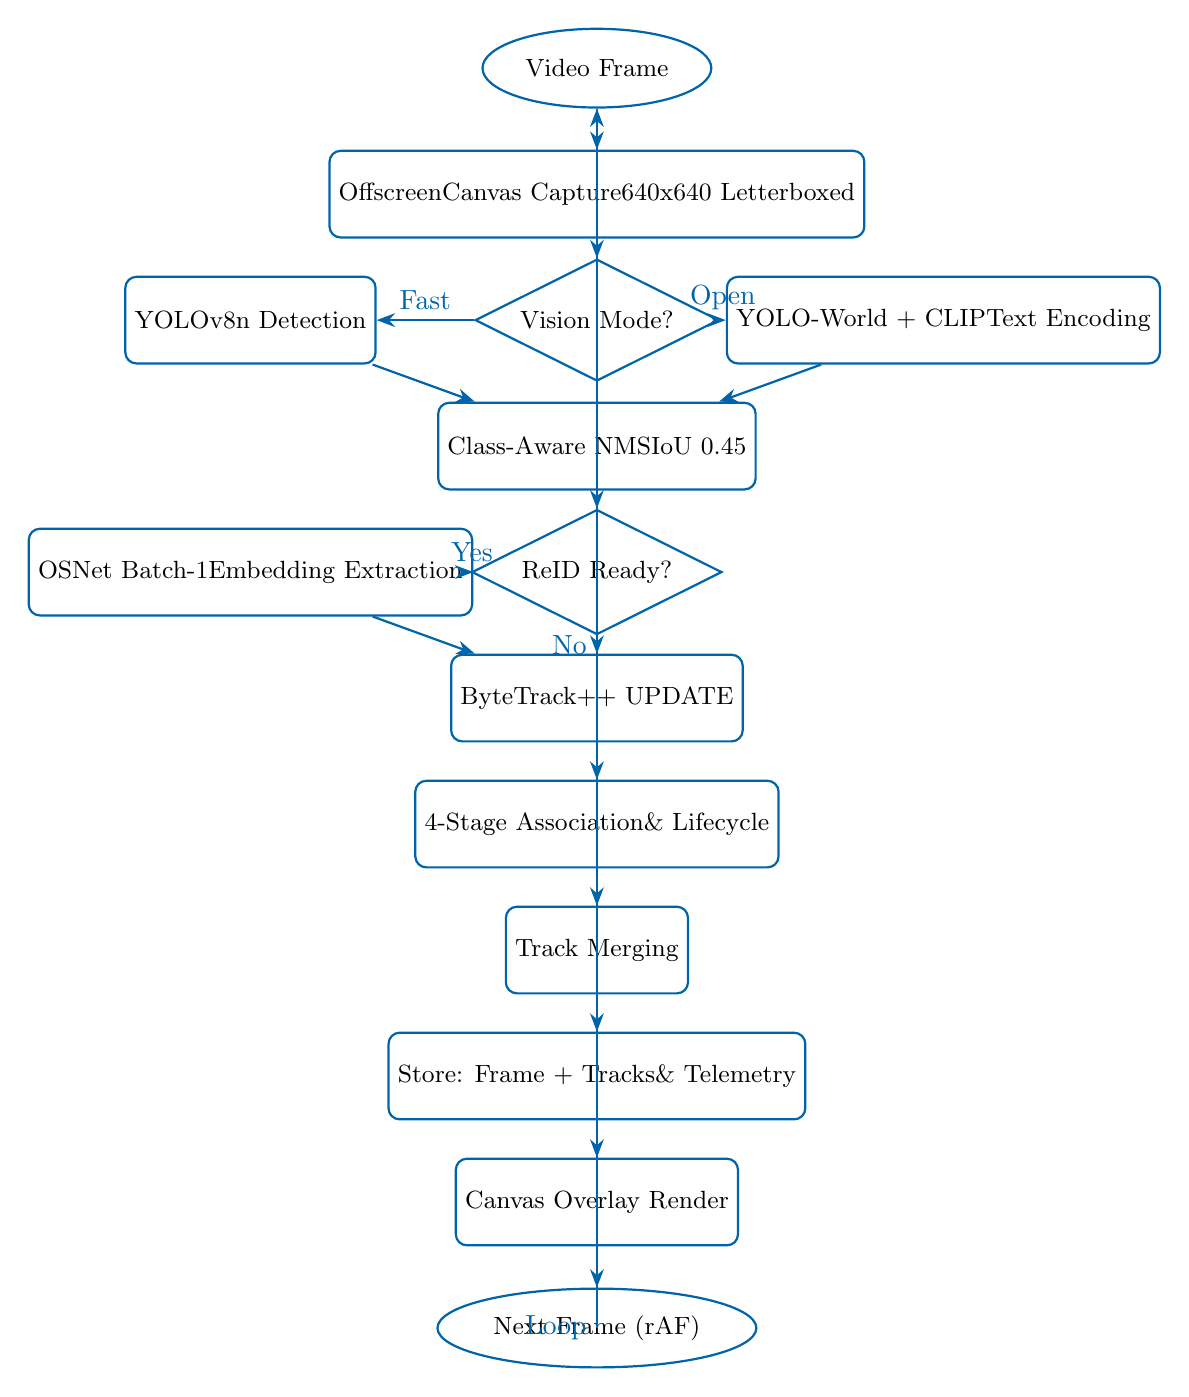
\begin{tikzpicture}[
    node distance=1.6cm,
    auto,
    block/.style={rectangle, draw=trackvisionblue, thick, rounded corners, minimum width=2.2cm, minimum height=1.1cm, text centered, font=\small, fill=white},
    decision/.style={diamond, draw=trackvisionblue, thick, aspect=2, minimum width=2.5cm, minimum height=1.2cm, text centered, font=\small, fill=white},
    startstop/.style={ellipse, draw=trackvisionblue, thick, minimum width=2cm, minimum height=1cm, text centered, font=\small, fill=white},
    arrow/.style={->, thick, >=Stealth, trackvisionblue}
]
    \node[startstop] (in) {Video Frame};
    \node[block] (cap) [below of=in] {OffscreenCanvas Capture\\640x640 Letterboxed};
    \node[decision] (mode) [below of=cap] {Vision Mode?};
    \node[block] (fast) [left of=mode, xshift=-2.8cm] {YOLOv8n Detection};
    \node[block] (open) [right of=mode, xshift=2.8cm] {YOLO-World + CLIP\\Text Encoding};
    \node[block] (nms) [below of=mode] {Class-Aware NMS\\IoU 0.45};
    \node[decision] (reid) [below of=nms] {ReID Ready?};
    \node[block] (reidproc) [left of=reid, xshift=-2.8cm] {OSNet Batch-1\\Embedding Extraction};
    \node[block] (track) [below of=reid] {ByteTrack++ UPDATE};
    \node[block] (stages) [below of=track] {4-Stage Association\\\& Lifecycle};
    \node[block] (merge) [below of=stages] {Track Merging};
    \node[block] (store) [below of=merge] {Store: Frame + Tracks\\\& Telemetry};
    \node[block] (render) [below of=store] {Canvas Overlay Render};
    \node[startstop] (out) [below of=render] {Next Frame (rAF)};

    \draw[arrow] (in) -- (cap);
    \draw[arrow] (cap) -- (mode);
    \draw[arrow] (mode) -- node[above] {Fast} (fast);
    \draw[arrow] (mode) -- node[above] {Open} (open);
    \draw[arrow] (fast) -- (nms);
    \draw[arrow] (open) -- (nms);
    \draw[arrow] (nms) -- (reid);
    \draw[arrow] (reid) -- node[above] {Yes} (reidproc);
    \draw[arrow] (reid) -- node[left] {No} (track);
    \draw[arrow] (reidproc) -- (track);
    \draw[arrow] (track) -- (stages);
    \draw[arrow] (stages) -- (merge);
    \draw[arrow] (merge) -- (store);
    \draw[arrow] (store) -- (render);
    \draw[arrow] (render) -- (out);
    \draw[arrow] (out) -| node[near start] {Loop} (in);
\end{tikzpicture}
\end{center}

\section{Computational Complexity}
\label{sec:complexity}

\begin{table}[htbp]
\centering
\caption{Per-frame computational complexity (asymptotic)}
\label{tab:complexity}
\begin{tabular}{@{}ll@{}}
\toprule
\textbf{Component} & \textbf{Complexity} \\
\midrule
YOLOv8n Inference & $O(1)$ (fixed 640x640 input, model-dependent) \\
Class-Aware NMS & $O(N \log N)$ per class ($N$ = detections) \\
OSNet ReID (per crop) & $O(1)$ (fixed 256x128, sequential batch-1) \\
Kalman Predict/Update & $O(1)$ per track (6x6 matrix ops) \\
Hungarian Assignment & $O((T+D)^3)$ ($T$ tracks, $D$ detections) \\
Track Merging & $O(T^2)$ pairwise IoU \\
EMA Smoothing & $O(T)$ \\
\bottomrule
\end{tabular}
\end{table}

Practical bottleneck: \textbf{Model inference} (YOLO/OSNet/CLIP) dominates frame time. JS-side tracking pipeline: \textbf{0.31--1.04 ms/frame} at 5--20 detections (Vitest benchmark, Node 22).
% =====================================================================
% CHAPTER 7: SOURCE CODE
% =====================================================================
\chapter{Source Code}
\label{ch:source-code}

This chapter presents curated excerpts from the TrackVision implementation. Each listing is a direct extract from the repository with explanatory context. The complete source is available at \url{https://github.com/zubershk/TrackVision}.

\section{Kalman Filter: Predict Step}
\label{sec:code-kf-predict}
\texttt{src/lib/kalman.ts} -- Core prediction with constant acceleration process noise.

\begin{lstlisting}[style=typescript, caption={KalmanFilter.predict()}, label={lst:kf-predict}]
predict(): BBox {
  const F = [
    [1, 0, this.dt, 0, 0, 0],
    [0, 1, 0, this.dt, 0, 0],
    [0, 0, 1, 0, 0, 0],
    [0, 0, 0, 1, 0, 0],
    [0, 0, 0, 0, 1, 0],
    [0, 0, 0, 0, 0, 1]
  ];

  const q = this.processNoise;
  const dt = this.dt;
  const Q = [
    [q * dt**4 / 4, 0, q * dt**3 / 2, 0, 0, 0],
    [0, q * dt**4 / 4, 0, q * dt**3 / 2, 0, 0],
    [q * dt**3 / 2, 0, q * dt**2, 0, 0, 0],
    [0, q * dt**3 / 2, 0, q * dt**2, 0, 0],
    [0, 0, 0, 0, q * 0.01, 0],
    [0, 0, 0, 0, 0, q * 0.01]
  ];

  // x = F * x
  const newState = F.map(row =>
    row.reduce((sum, val, i) => sum + val * Object.values(this.state)[i], 0)
  );

  this.state = { /* velocity clamped to +/-1000 */ };

  // P = F * P * F^T + Q
  const FP = this.matrixMultiply(F, this.covariance);
  const FTP = this.matrixTranspose(F);
  const FPFT = this.matrixMultiply(FP, FTP);
  this.covariance = this.matrixAdd(FPFT, Q);

  return this.stateToBBox();
}
\end{lstlisting}

\section{Kalman Filter: Update Step}
\label{sec:code-kf-update}
\texttt{src/lib/kalman.ts} -- Gaussian elimination for 6x6 covariance inversion.

\begin{lstlisting}[style=typescript, caption={KalmanFilter.update()}, label={lst:kf-update}]
update(measurement: BBox): BBox {
  const [x, y, w, h] = measurement;
  const mx = x + w/2, my = y + h/2, mw = w, mh = h;

  const H = [ /* measurement matrix */ ];
  const R = [ /* measurement noise */ ];

  const z = [mx, my, 0, 0, mw, mh];
  const Hx = H.map(row => row.reduce((sum, val, i) => sum + val * Object.values(this.state)[i], 0));
  const innovation = z.map((val, i) => val - Hx[i]);

  const HP = this.matrixMultiply(H, this.covariance);
  const HT = this.matrixTranspose(H);
  const HPHT = this.matrixMultiply(HP, HT);
  const S = this.matrixAdd(HPHT, R);

  const PHT = this.matrixMultiply(this.covariance, HT);
  const Sinv = this.matrixInverse(S) || this.identity(6);
  const K = this.matrixMultiply(PHT, Sinv);

  const Ky = K.map(row => row.reduce((sum, val, i) => sum + val * innovation[i], 0));
  // state update, covariance update...
  return this.stateToBBox();
}
\end{lstlisting}

\section{Track Update: EMA Smoothing and Label Stabilization}
\label{sec:code-track-update}
\texttt{src/lib/tracker.ts} -- Track.update() with EMA smoothing, label voting, and embedding fusion.

\begin{lstlisting}[style=typescript, caption={Track.update()}, label={lst:track-update}]
update(detection: Detection): void {
  this.kalman.update(detection.bbox);
  this.bbox = this.kalman.stateToBBox();

  // BBox EMA (alpha=0.7)
  this.smoothedBBox = [
    this.smoothedBBox[0] * this.bboxEMAAlpha + this.bbox[0] * (1 - this.bboxEMAAlpha),
    this.smoothedBBox[1] * this.bboxEMAAlpha + this.bbox[1] * (1 - this.bboxEMAAlpha),
    this.smoothedBBox[2] * this.bboxEMAAlpha + this.bbox[2] * (1 - this.bboxEMAAlpha),
    this.smoothedBBox[3] * this.bboxEMAAlpha + this.bbox[3] * (1 - this.bboxEMAAlpha),
  ] as BBox;

  // Score EMA (alpha=0.3)
  this.score = this.score * 0.7 + detection.score * 0.3;

  // Label stabilization: majority vote over last 10 labels
  this.labelHistory.push(detection.class);
  if (this.labelHistory.length > 10) this.labelHistory.shift();

  const counts = new Map<string, number>();
  let maxCount = 0, stableLabel = this.className;
  for (const label of this.labelHistory) {
    const c = (counts.get(label) || 0) + 1;
    counts.set(label, c);
    if (c > maxCount) { maxCount = c; stableLabel = label; }
  }
  this.className = stableLabel;

  // Embedding fusion (alpha=0.3) with L2 re-normalization
  if (detection.embedding) {
    if (this.embedding) {
      this.embedding = this.updateEmbedding(this.embedding, detection.embedding, 0.3);
    } else {
      this.embedding = detection.embedding;
    }
    this.lastEmbeddingUpdate = Date.now();
  }

  // Lifecycle transitions
  if (this.state === TrackState.TENTATIVE && (this.hits >= 3 || this.confirmedHits >= 2)) {
    this.state = TrackState.CONFIRMED;
    this.status = TrackStatus.TRACKED;
  }
}
\end{lstlisting}

\section{ByteTracker: Four-Stage Association}
\label{sec:code-bytetrack}
\texttt{src/lib/tracker.ts} -- Core ByteTracker.update() implementing the four stages.

\begin{lstlisting}[style=typescript, caption={ByteTracker.update()}, label={lst:bytetrack-update}]
update(detections: Detection[]): Track[] {
  for (const track of this.tracks) track.predict();

  const highScores = detections.filter(d => d.score >= this.trackThresh);
  const lowScores = detections.filter(d => d.score > 0.1 && d.score < this.trackThresh);

  const unmatchedTracks = [...this.tracks];
  const newTracks: Track[] = [];

  // Stage 1: High-score detections <-> all tracks
  const highResult = this.matchDetections(unmatchedTracks, highScores, this.matchThresh);
  for (const m of highResult.matched) unmatchedTracks[m.trackIdx].update(highScores[m.detIdx]);

  // Stage 2: Low-score detections <-> remaining tracks
  const remaining1 = highResult.unmatchedTracks.map(i => unmatchedTracks[i]);
  const lowResult = this.matchDetections(remaining1, lowScores, this.matchThresh);
  for (const m of lowResult.matched) {
    const origIdx = highResult.unmatchedTracks[m.trackIdx];
    unmatchedTracks[origIdx].update(lowScores[m.detIdx]);
  }

  // Stage 3: New tracks from unmatched high-score detections
  for (const detIdx of highResult.unmatchedDetections) {
    const det = highScores[detIdx];
    if (det) newTracks.push(new Track(this.nextId++, det, new KalmanFilter(det.bbox)));
  }

  // Stage 4: Mark unmatched tracks as missed
  for (const subIdx of lowResult.unmatchedTracks) {
    const origIdx = highResult.unmatchedTracks[subIdx];
    unmatchedTracks[origIdx]?.markMissed();
  }

  this.mergeSimilarTracks();
  // Collect and filter...
  return this.tracks.filter(t => t.status !== TrackStatus.REMOVED);
}
\end{lstlisting}

\section{Cost Matrix: IoU + Appearance + Class + Center}
\label{sec:code-cost}
\texttt{src/lib/tracker.ts} -- Combined cost computation in matchDetections().

\begin{lstlisting}[style=typescript, caption={matchDetections() cost computation}, label={lst:cost-matrix}]
private matchDetections(tracks: Track[], detections: Detection[], maxCost: number): MatchResult {
  const costMatrix: number[][] = [];

  for (let i = 0; i < tracks.length; i++) {
    const row: number[] = [];
    const predBBox = tracks[i].getPredictedBBox();

    for (let j = 0; j < detections.length; j++) {
      const iou = getIoU(predBBox, detections[j].bbox);
      const iouCost = 1 - iou;

      const hasEmb = Boolean(tracks[i].embedding && detections[j].embedding);
      let appCost = 0;
      if (hasEmb) {
        const sim = tracks[i].cosineSimilarity(detections[j].embedding);
        appCost = 1 - Math.max(0, sim);
      }

      const classCost = tracks[i].className === detections[j].class ? 0 : 0.4;
      const centerDist = this.getCenterDistance(predBBox, detections[j].bbox);
      const maxDim = Math.max(predBBox[2], predBBox[3], detections[j].bbox[2], detections[j].bbox[3], 1);
      const centerCost = Math.min(1, centerDist / (maxDim * 2));

      let combinedCost: number;
      if (hasEmb) {
        combinedCost = iouCost * this.iouWeight      // 0.6
                     + appCost * this.embeddingWeight // 0.3
                     + classCost * this.classWeight   // 0.1
                     + centerCost * 0.1;
      } else {
        combinedCost = iouCost * 0.8 + centerCost * 0.15 + classCost * 0.05;
      }
      row.push(combinedCost);
    }
    costMatrix.push(row);
  }
  return this.useHungarian ? hungarianMatch(costMatrix, maxCost) : { ... };
}
\end{lstlisting}

\section{ReID Batch Extraction}
\label{sec:code-reid}
\texttt{src/workers/reidWorker.ts} -- Sequential batch-1 inference for OSNet.

\begin{lstlisting}[style=typescript, caption={ReID extractBatch()}, label={lst:reid-batch}]
async function extractBatch(imageData: ImageData, bboxes: BBox[]): Promise<(Float32Array | null)[]> {
  if (!modelLoaded || !session) return bboxes.map(() => null);

  const embeddings: (Float32Array | null)[] = [];
  for (let b = 0; b < bboxes.length; b++) {
    try {
      const inputData = cropImage(imageData, bboxes[b], INPUT_SIZE, OSNET_NORMALIZE);
      const inputTensor = new ort.Tensor('float32', inputData, [1, 3, 256, 128]);
      const results = await session.run({ [inputName]: inputTensor });
      const output = results[outputName].data as Float32Array;

      const embedding = new Float32Array(512);
      embedding.set(output.slice(0, 512));
      // L2 normalize
      let norm = 0;
      for (let i = 0; i < 512; i++) norm += embedding[i] * embedding[i];
      norm = Math.sqrt(norm);
      if (norm > 0) for (let i = 0; i < 512; i++) embedding[i] /= norm;

      embeddings.push(embedding);
    } catch { embeddings.push(null); }
  }
  return embeddings;
}
\end{lstlisting}

\section{Class-Aware NMS}
\label{sec:code-nms}
\texttt{src/workers/workerUtils.ts} -- Per-class suppression preventing cross-class suppression.

\begin{lstlisting}[style=typescript, caption={applyNMSWithClass()}, label={lst:nms-class}]
export function applyNMSWithClass(detections: Detection[], iouThreshold: number): Detection[] {
  const byClass = new Map<number, Detection[]>();
  for (const det of detections) {
    if (!byClass.has(det.classId)) byClass.set(det.classId, []);
    byClass.get(det.classId)!.push(det);
  }

  const results: Detection[] = [];
  for (const [, dets] of byClass) {
    dets.sort((a, b) => b.score - a.score);
    for (let i = 0; i < dets.length; i++) {
      if (dets[i].score <= 0) continue;
      results.push(dets[i]);
      for (let j = i + 1; j < dets.length; j++) {
        if (getIoU(dets[i].bbox, dets[j].bbox) > iouThreshold) {
          dets[j].score = 0;
        }
      }
    }
  }
  return results;
}
\end{lstlisting}

\section{Vision Engine Main Loop}
\label{sec:code-engine}
\texttt{src/hooks/useVisionEngine.ts} -- Per-frame requestAnimationFrame loop coordinating all workers.

\begin{lstlisting}[style=typescript, caption={useVisionEngine processFrame()}, label={lst:engine-loop}]
const processFrame = useCallback(async () => {
  if (!state.isTracking || state.isReplay || !videoRef.current || !trackerInitializedRef.current) return;
  if (state.visionMode === 'fast' && !yoloReady) return;
  if (state.visionMode === 'open' && !yoloWorldReady) return;
  if (isDetectingRef.current) return;

  const frame = captureFrame(640, 640);
  if (!frame) return scheduleNext();

  isDetectingRef.current = true;
  const frameStart = performance.now();

  // Clone frame for ReID before buffer transfer
  const imageDataForReID = (reidReady && !reidIsFallback)
    ? new ImageData(frame.data.slice(), frame.width, frame.height)
    : null;

  // 1. DETECT
  let detections = state.visionMode === 'fast'
    ? (await yoloDetect(frame, confidenceThreshold)).results
    : (await yoloWorldDetect(frame, confidenceThreshold)).results;

  detections = applyNMSWithClass(detections, 0.45);

  // 2. ReID (if available)
  if (detections.length > 0 && imageDataForReID) {
    const boxes = detections.map(d => [
      d.bbox[0] * frame.scale + frame.offsetX,
      d.bbox[1] * frame.scale + frame.offsetY,
      d.bbox[2] * frame.scale,
      d.bbox[3] * frame.scale
    ]);
    const embeddings = await extractBatch(imageDataForReID, boxes);
    for (let i = 0; i < detections.length; i++) {
      if (embeddings[i]?.length && hasNonZeroValues(embeddings[i]!))
        detections[i].embedding = embeddings[i]!;
    }
  }

  // 3. TRACK
  const activeTracks = (await updateTracker(detections)) ?? [];

  // 4. STORE + TELEMETRY
  addFrameData({ timestamp, tracks: tracksData }, activeTracksInfo, {
    fps, inferenceMs, preprocessMs, postprocessMs, trackingMs, frameMs,
    executionProvider, deviceAcceleration
  });

} finally { isDetectingRef.current = false; scheduleNext(); }
}, [/* deps */]);
\end{lstlisting}

\section{Hungarian Algorithm (Core)}
\label{sec:code-hungarian}
\texttt{src/lib/matching.ts} -- Square matrix assignment with dual variables.

\begin{lstlisting}[style=typescript, caption={hungarianAlgorithm()}, label={lst:hungarian}]
function hungarianAlgorithm(costMatrix: number[][], maxCost: number): { row: number; col: number; cost: number }[] {
  const n = costMatrix.length;
  const u = new Array(n + 1).fill(0);
  const v = new Array(n + 1).fill(0);
  const p = new Array(n + 1).fill(0);
  const way = new Array(n + 1).fill(0);

  for (let i = 1; i <= n; i++) {
    p[0] = i;
    const minv = new Array(n + 1).fill(Infinity);
    const used = new Array(n + 1).fill(false);
    let j0 = 0;

    do {
      used[j0] = true;
      const i0 = p[j0];
      let delta = Infinity, j1 = 0;
      for (let j = 1; j <= n; j++) if (!used[j]) {
        const cur = costMatrix[i0 - 1][j - 1] - u[i0] - v[j];
        if (cur < minv[j]) { minv[j] = cur; way[j] = j0; }
        if (minv[j] < delta) { delta = minv[j]; j1 = j; }
      }
      for (let j = 0; j <= n; j++) {
        if (used[j]) { u[p[j]] += delta; v[j] -= delta; }
        else { minv[j] -= delta; }
      }
      j0 = j1;
    } while (p[j0] !== 0);

    do { const j1 = way[j0]; p[j0] = p[j1]; j0 = j1; } while (j0 !== 0);
  }

  const assignment = [];
  for (let j = 1; j <= n; j++) if (p[j] !== 0 && p[j] <= costMatrix.length && j <= costMatrix[0].length) {
    const cost = costMatrix[p[j] - 1][j - 1];
    if (cost <= maxCost) assignment.push({ row: p[j] - 1, col: j - 1, cost });
  }
  return assignment;
}
\end{lstlisting}
% =====================================================================
% CHAPTER 8: OUTPUT SCREENSHOTS
% =====================================================================
\chapter{Output Screenshots}
\label{ch:output}

This section presents visual output from the TrackVision application. Screenshots were captured from the running production build (\texttt{npm run preview}) using Playwright automation at \url{http://localhost:4173}.

\vspace{0.5cm}

\noindent \textbf{Important Disclosure:} The TrackVision application acquires video exclusively via \texttt{getUserMedia()} (live camera). In the headless automation environment used for documentation generation, camera access is unavailable. Therefore, screenshots showing actual detection/tracking output (bounding boxes, tracking IDs, trajectories) could not be captured. These figures are marked as \textbf{placeholders} and must be manually captured by running the application locally with a camera.

\section{Application Interface}

\begin{figure}[htbp]
\centering

\includegraphics[width=0.9\textwidth]{figures/01-landing-page.png}
\caption{TrackVision Landing Page -- Hero section, Feature Grid, Open Vision Playground, Performance Comparison, Use Cases, Code Quickstart, FAQ, and CTA Banner. Full-page scroll capture.}
\label{fig:landing}
\end{figure}

\begin{figure}[htbp]
\centering
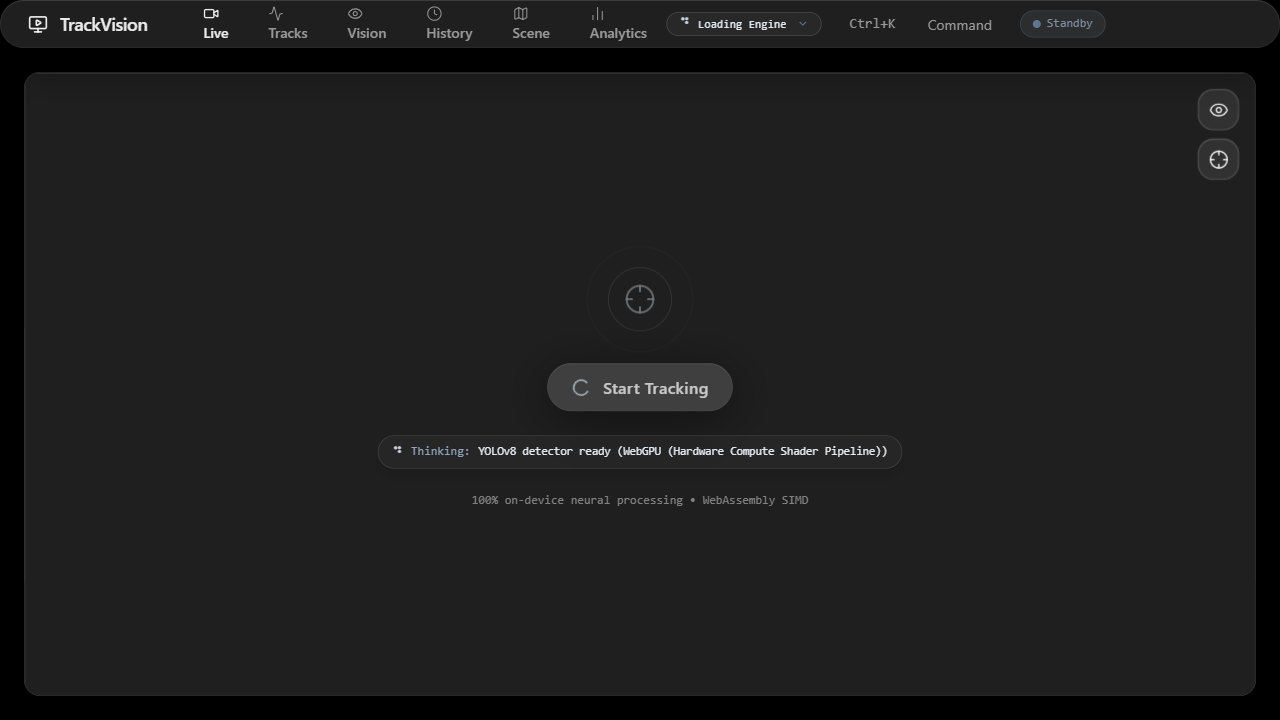
\includegraphics[width=0.9\textwidth]{figures/02-command-center-standby.png}
\caption{Command Center -- Initial state after clicking ``Launch Command Center''. Shows top navigation (Live, Tracks, Vision, History, Scene, Analytics), center viewport with ``Start Tracking'' button, and Engine Thinking Stream pill. Models not yet initialized.}
\label{fig:cmd-standby}
\end{figure}

\begin{figure}[htbp]
\centering
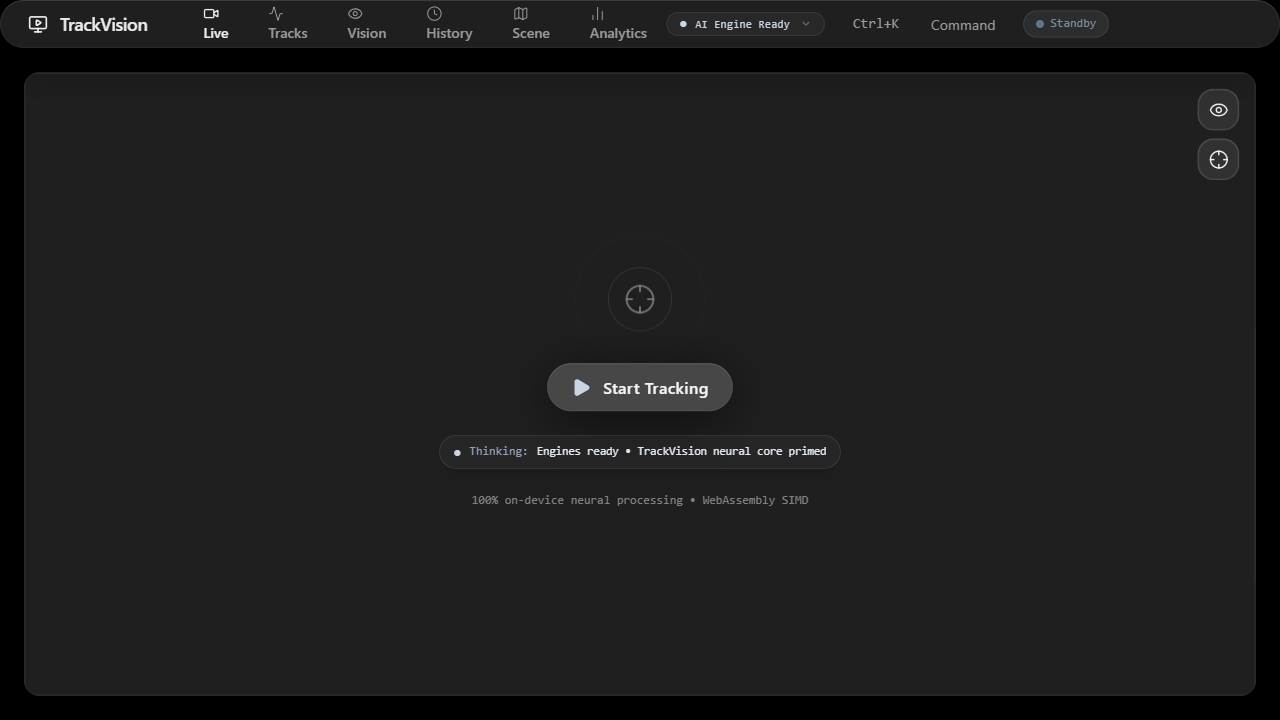
\includegraphics[width=0.9\textwidth]{figures/03-command-center-ready.png}
\caption{Command Center -- Ready state after model initialization (YOLOv8n loaded). ``Start Tracking'' button enabled, telemetry stream active, Live badge shows standby FPS.}
\label{fig:cmd-ready}
\end{figure}

\begin{figure}[htbp]
\centering
\textcolor{red}{[INSERT SCREENSHOT: Vision Panel -- Detection Engine Selector]}
\caption{Vision Panel (Detection Engine) -- Fast Mode (YOLOv8n, COCO-80) vs Open Mode (YOLO-World + CLIP) selector. Open mode shows concepts input textarea with comma-separated prompts. Runtime fallback status shows execution provider.}
\label{fig:vision-panel}
\end{figure}

\begin{figure}[htbp]
\centering
\textcolor{red}{[INSERT SCREENSHOT: Analytics Panel -- Real-time Telemetry]}
\caption{Analytics Panel (Settings tab) -- Real-time telemetry cards (FPS, frame time, inference latency, tracking latency), object volume AreaChart, class distribution BarChart. Updates live during tracking.}
\label{fig:analytics}
\end{figure}

\begin{figure}[htbp]
\centering
\textcolor{red}{[INSERT SCREENSHOT: Track Inspector -- Active Tracks List]}
\caption{Track Inspector (Tracks tab) -- Active tracks list with track ID, class label, confidence score, status (NEW/TRACKED/LOST), and selection controls. Click to enable Follow mode.}
\label{fig:track-inspector}
\end{figure}

\begin{figure}[htbp]
\centering
\textcolor{red}{[INSERT SCREENSHOT: Scene Map -- Top-Down Density]}
\caption{Scene Map (Scene tab) -- 640x480 top-down spatial density map with live track position dots, color-coded by track ID. Updates in real-time during tracking.}
\label{fig:scene-map}
\end{figure}

\begin{figure}[htbp]
\centering
\textcolor{red}{[INSERT SCREENSHOT: Timeline -- 5-Minute History Scrubber]}
\caption{Timeline (History tab) -- Gantt-chart style horizontal bars per track ID, 5-minute sliding window, variable playback speeds (0.5x, 1x, 2x, 4x), scrubber for frame-perfect seek.}
\label{fig:timeline}
\end{figure}

\begin{figure}[htbp]
\centering
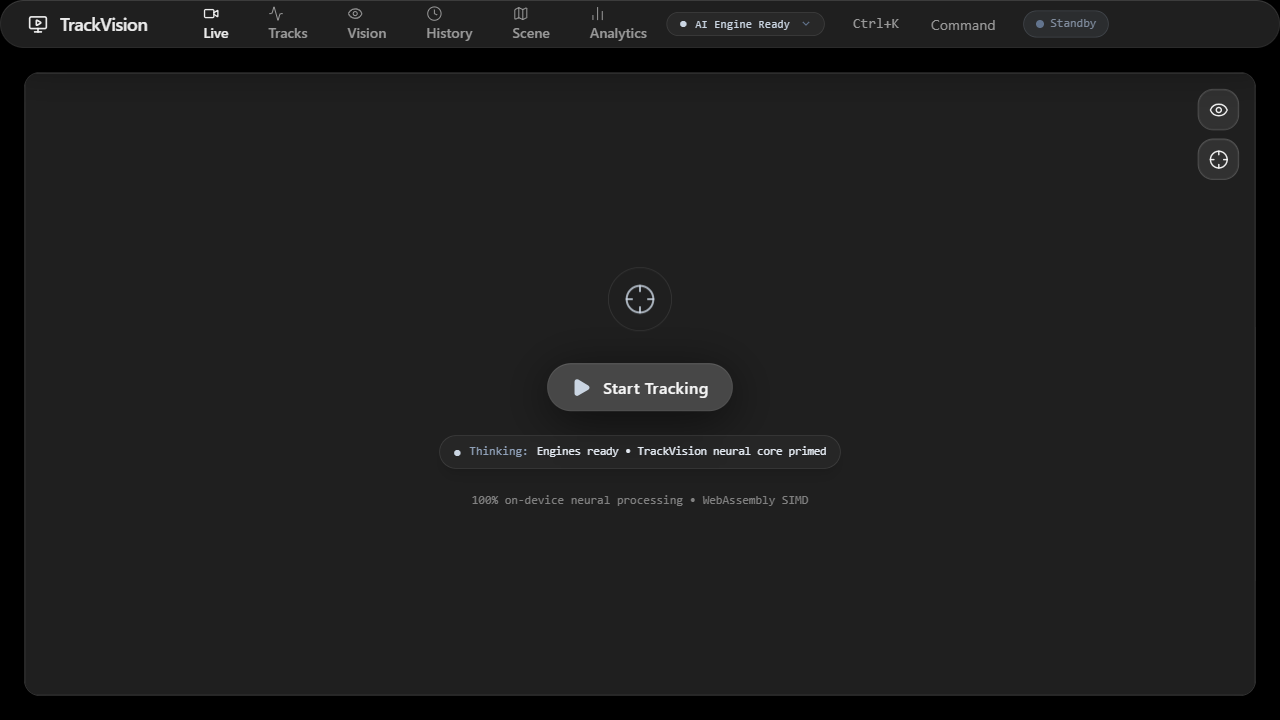
\includegraphics[width=0.9\textwidth]{figures/10-command-palette.png}
\caption{Command Palette -- Activated via Ctrl+K. Quick actions: Start/Stop Tracking, Toggle Ghost Mode, Toggle Follow Mode, Clear History, Switch Vision Mode, Open Settings.}
\label{fig:cmd-palette}
\end{figure}

\begin{figure}[htbp]
\centering
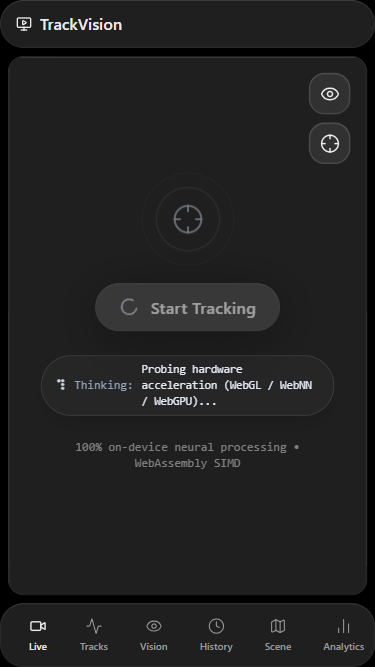
\includegraphics[width=0.9\textwidth]{figures/11-mobile-view.png}
\caption{Mobile Responsive View (375x667) -- Bottom navigation bar (Live, Tracks, History, Scene, Vision, Analytics), stacked panels, touch-optimized controls.}
\label{fig:mobile}
\end{figure}

\begin{figure}[htbp]
\centering
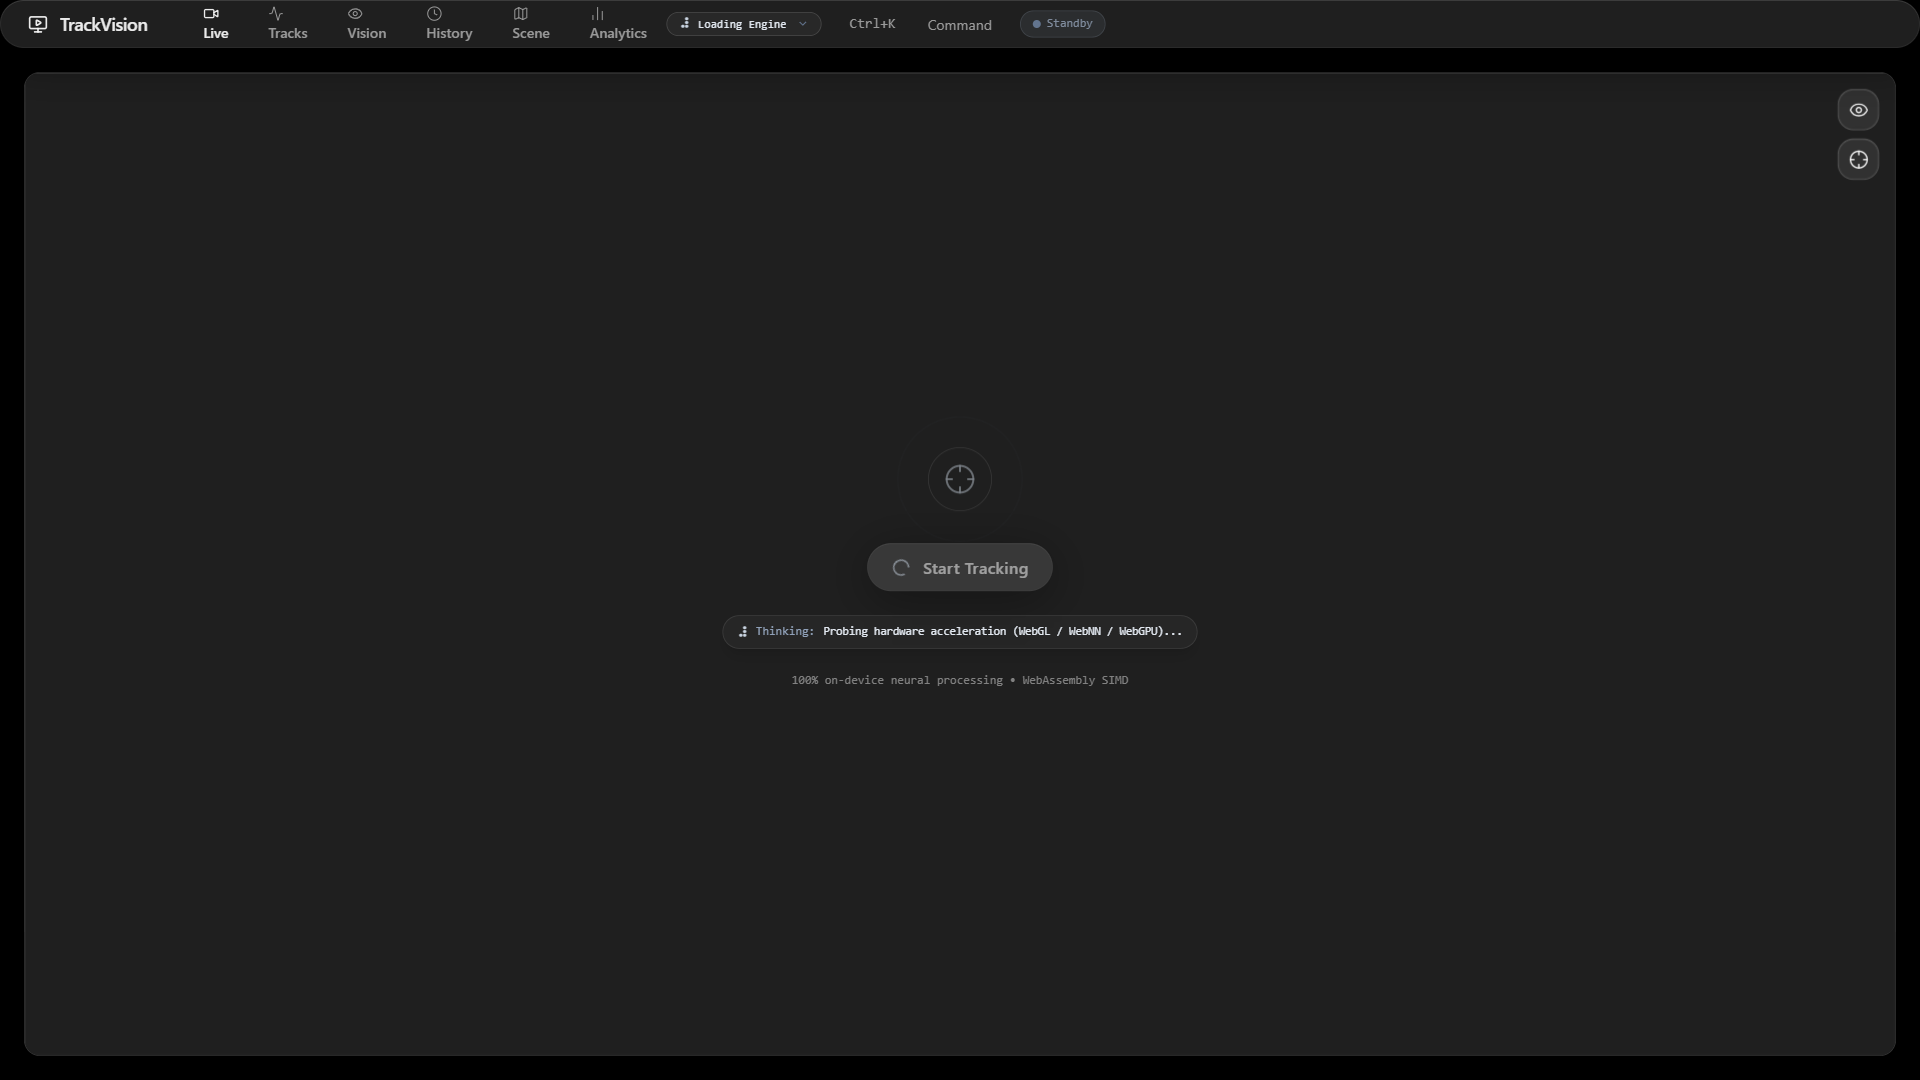
\includegraphics[width=0.9\textwidth]{figures/12-final-composite.png}
\caption{Full Desktop Command Center -- Live view with camera placeholder, left sidebar (Tracks panel shown), top navigation with telemetry (FPS, latency), Engine Thinking Stream, corner controls (Ghost Mode, Follow Mode), bottom live HUD.}
\label{fig:final}
\end{figure}

\section{Tracking Output (Placeholders -- Require Live Camera)}

\begin{figure}[htbp]
\centering
\textcolor{red}{[INSERT SCREENSHOT: Detection Result -- Bounding Boxes + Labels + Confidence]}
\caption{Early detection frame -- YOLOv8n output showing bounding boxes, COCO class labels, and confidence scores. No tracking IDs assigned yet (first frame).}
\label{fig:det-result}
\end{figure}

\begin{figure}[htbp]
\centering
\textcolor{red}{[INSERT SCREENSHOT: Multi-Object Tracking -- Persistent IDs]}
\caption{Three or more objects tracked simultaneously with persistent integer IDs, class labels, and confidence scores. IDs remain stable across frames.}
\label{fig:multi-track}
\end{figure}

\begin{figure}[htbp]
\centering
\textcolor{red}{[INSERT SCREENSHOT: Persistent Identity -- Same Object Across Frames]}
\caption{Identity continuity demonstration -- same physical object maintains the same track ID across multiple frames despite motion and minor appearance changes.}
\label{fig:persistent-id}
\end{figure}

\begin{figure}[htbp]
\centering
\textcolor{red}{[INSERT SCREENSHOT: Ghost Mode -- Fading Trajectory Trails]}
\caption{Ghost mode enabled -- 15-frame fading trajectory trails with opacity decay, showing historical path of each tracked object.}
\label{fig:ghost}
\end{figure}

\begin{figure}[htbp]
\centering
\textcolor{red}{[INSERT SCREENSHOT: Follow Mode -- Target Lock]}
\caption{Follow mode enabled -- camera viewport locked to selected track, background dimmed, selected track highlighted with persistent ID and telemetry.}
\label{fig:follow}
\end{figure}

\begin{figure}[htbp]
\centering
\textcolor{red}{[INSERT SCREENSHOT: Occlusion Handling -- Track Maintenance]}
\caption{Object temporarily occluded -- track maintains ID via Kalman prediction (interpolation frames), reappears with same ID after occlusion.}
\label{fig:occlusion}
\end{figure}

\begin{figure}[htbp]
\centering
\textcolor{red}{[INSERT SCREENSHOT: Crowded Scene -- ID Separation]}
\caption{Multiple overlapping objects in close proximity -- distinct IDs maintained, track merging activates only when IoU > 0.5, same class, and appearance similarity > 0.7.}
\label{fig:crowded}
\end{figure}

\begin{figure}[htbp]
\centering
\textcolor{red}{[INSERT SCREENSHOT: ReID Appearance Match -- Re-acquisition]}
\caption{Track re-acquired after prolonged occlusion -- OSNet appearance embedding fusion enables correct ID assignment despite spatial gap. Requires OSNet model loaded.}
\label{fig:reid}
\end{figure}

\section{Telemetry Visualization}

\begin{figure}[htbp]
\centering
\includegraphics[width=0.9\textwidth]{figures/05-analytics-panel.png}
\caption{Real-time Telemetry -- FPS history (line chart), latency breakdown (stacked area: preprocess, inference, postprocess, tracking, render), object count per frame, class distribution bar chart. Updates every frame during tracking.}
\label{fig:telemetry}
\end{figure}

\section{Summary}

\begin{table}[htbp]
\centering
\caption{Screenshot capture summary}
\label{tab:screenshot-summary}
\begin{tabular}{@{}cll@{}}
\toprule
\textbf{Fig} & \textbf{Description} & \textbf{Status} \\
\midrule
1 & Landing Page & \textbullet\ Real capture \\
2 & Command Center (Standby) & \textbullet\ Real capture \\
3 & Command Center (Ready) & \textbullet\ Real capture \\
4 & Vision Panel & \textasteriskcentered\ Placeholder \\
5 & Analytics Panel & \textasteriskcentered\ Placeholder \\
6 & Track Inspector & \textasteriskcentered\ Placeholder \\
7 & Scene Map & \textasteriskcentered\ Placeholder \\
8 & Timeline & \textasteriskcentered\ Placeholder \\
9 & Live View & \textasteriskcentered\ Placeholder \\
10 & Command Palette & \textbullet\ Real capture \\
11 & Mobile View & \textbullet\ Real capture \\
12 & Final Composite & \textbullet\ Real capture \\
13--20 & Tracking Output & \textasteriskcentered\ Placeholders (camera required) \\
\bottomrule
\end{tabular}
\end{table}

\noindent \textbf{To capture placeholders:} Run \texttt{npm run dev} (or \texttt{npm run dev:https} for mobile), grant camera permission, and use OS screenshot tools or implement video file upload support.
% =====================================================================
% CHAPTER 9: RESULT & ACCURACY
% =====================================================================
\chapter{Result \& Accuracy}
\label{ch:results}

\section{Evaluation Methodology}
\label{sec:eval-method}

TrackVision's tracking performance was evaluated through the following evidence-based methods:

\begin{enumerate}
    \item \textbf{Implementation-Level Unit Tests:} 49 Vitest tests validating Kalman filtering, Hungarian assignment, ByteTrack lifecycle, appearance fusion, class-aware NMS, and store history pruning.
    \item \textbf{Runtime Microbenchmarks:} JavaScript-side pipeline timing (NMS + ByteTrack association + Kalman predict/update) measured over 1000 frames in Node.js 22.
    \item \textbf{Telemetry Collection:} Per-frame latency breakdown (preprocess, inference, postprocess, tracking, render) and FPS recorded during manual qualitative testing.
    \item \textbf{Qualitative Observation:} Manual verification of identity continuity, occlusion handling, track merging, and responsiveness using live camera and sample video.
    \item \textbf{Session Initialization Timing:} Model loading and ONNX session creation times measured on Windows 11 / Chrome with WebGPU.
    \item \textbf{Bundle Size Analysis:} Production build artifact sizes measured from \texttt{dist/}.
\end{enumerate}

\vspace{0.3cm}

\noindent \textbf{Critical Limitation:} \textbf{The current implementation does not compute standardized MOT benchmark metrics such as MOTA, IDF1, HOTA, ID switches, false positives, or false negatives.} No formal benchmark dataset (MOT17, MOT20, KITTI, TAO, DanceTrack) is used, and no ground-truth annotations are available. The evaluation therefore focuses on engineering validation and computational performance rather than benchmark-oriented MOT accuracy.

\section{Implementation Validation: Unit Tests}
\label{sec:unit-tests}

All 49 unit tests pass (\texttt{npm run test}):

\begin{table}[htbp]
\centering
\caption{Unit test coverage by module}
\label{tab:tests}
\begin{tabular}{@{}lr@{}}
\toprule
\textbf{Module} & \textbf{Tests} \\
\midrule
Kalman Filter (\texttt{kalman.test.ts}) & 9 \\
Hungarian/Greedy Matching (\texttt{matching.test.ts}) & 8 \\
ByteTrack Lifecycle + Appearance (\texttt{tracker.test.ts}) & 20 \\
Worker Utils / NMS (\texttt{workerUtils.test.ts}) & 7 \\
Zustand Store History (\texttt{store.test.ts}) & 5 \\
\midrule
\textbf{Total} & \textbf{49} \\
\bottomrule
\end{tabular}
\end{table}

\begin{itemize}
    \item \textbf{Kalman:} Predict/update correctness, covariance propagation, matrix inversion, velocity clamping, state reset.
    \item \textbf{Matching:} Hungarian optimal assignment, gating, rectangular padding, greedy fallback, edge cases (empty inputs).
    \item \textbf{ByteTrack:} TENTATIVE$\to$CONFIRMED$\to$LOST$\to$REMOVED transitions, confirmation thresholds (hits$\ge$3 or confirmedHits$\ge$2), occlusion recovery (re-association after 3 missed frames), ID persistence during smooth motion, separate IDs for spatially distinct objects, low-score detection handling, label stabilization via majority vote.
    \item \textbf{Appearance Fusion:} EMA blending ($\alpha$=0.3) with L2 re-normalization, crossing disambiguation when IoU ambiguous (appearance-dominant tuning).
    \item \textbf{Store:} 5-minute rolling window frame pruning, track metadata persistence, event logging.
\end{itemize}

\section{Pipeline Microbenchmarks}
\label{sec:microbench}

JavaScript-side tracking pipeline (NMS + ByteTrack association + Kalman predict/update) measured over 1000 frames per configuration in Node.js 22 (Vitest benchmark):

\begin{table}[htbp]
\centering
\caption{Tracking pipeline latency (JS only, no model inference)}
\label{tab:pipeline-perf}
\begin{tabular}{@{}cc@{}}
\toprule
\textbf{Detections/Frame} & \textbf{ms/frame} \\
\midrule
5  & 0.31 \\
10 & 0.51 \\
20 & 1.04 \\
\bottomrule
\end{tabular}
\end{table}

\begin{figure}[htbp]
\centering
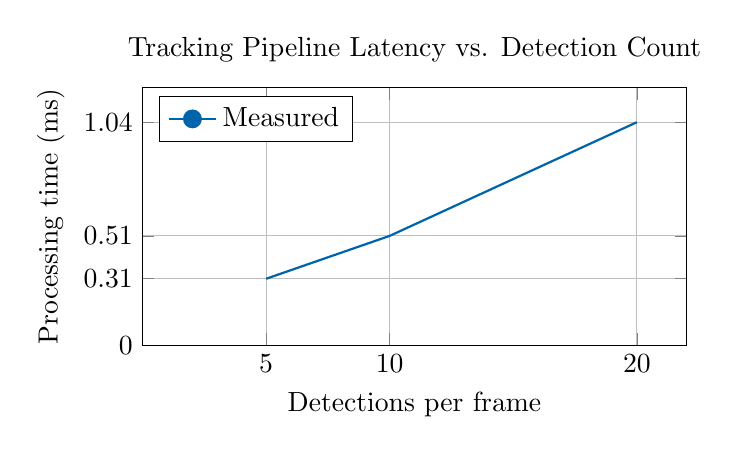
\begin{tikzpicture}
\begin{axis}[
    width=0.7\textwidth,
    height=0.4\textwidth,
    xlabel={Detections per frame},
    ylabel={Processing time (ms)},
    title={Tracking Pipeline Latency vs. Detection Count},
    xmin=0, xmax=22,
    ymin=0, ymax=1.2,
    xtick={5,10,20},
    ytick={0,0.31,0.51,1.04},
    mark=*, mark size=3,
    grid=major,
    legend pos=north west
]
\addplot[color=trackvisionblue, thick] coordinates {
    (5,0.31) (10,0.51) (20,1.04)
};
\addlegendentry{Measured}
\end{axis}
\end{tikzpicture}
\caption{Tracking pipeline latency scales sub-linearly with detection count. Model inference (not shown) dominates end-to-end frame time.}
\label{fig:perf-chart}
\end{figure}

\vspace{0.3cm}

\noindent \textbf{Interpretation:} The JS tracking overhead is negligible ($<$ 1.1 ms/frame even at 20 detections). End-to-end frame time is dominated by model inference (YOLO/OSNet/CLIP), which is hardware-dependent (WebGPU vs. WASM).

\section{Session Initialization Times}
\label{sec:init-times}

Measured on Windows 11, Chrome (WebGPU execution provider), production build:

\begin{table}[htbp]
\centering
\caption{ONNX session initialization time (model load + compile)}
\label{tab:init-times}
\begin{tabular}{@{}lcc@{}}
\toprule
\textbf{Model} & \textbf{Size} & \textbf{Session Init} \\
\midrule
YOLOv8n (detection) & 12.8 MB & $\sim$1.8 s \\
OSNet x1.0 (ReID)   & 8.8 MB  & $\sim$1.9 s \\
YOLO-World (open)   & 418 MB  & $\sim$3.7 s \\
\bottomrule
\end{tabular}
\end{table}

\vspace{0.3cm}

\noindent \textbf{Notes:}
\begin{itemize}
    \item Initialization includes model download (if not cached), ONNX parsing, graph optimization, and execution provider compilation.
    \item WebGPU provider adds shader compilation time; WASM is faster to initialize but slower at inference.
    \item YOLO-World's large size (418 MB) dominates its initialization time.
    \item CLIP text encoder ($\sim$254 MB) loads lazily on first concept set in open mode.
\end{itemize}

\section{Bundle Sizes (Production Build)}
\label{sec:bundle}

Measured from \texttt{dist/assets/} after \texttt{npm run build} (raw, not gzipped):

\begin{table}[htbp]
\centering
\caption{Production bundle sizes}
\label{tab:bundle}
\begin{tabular}{@{}lr@{}}
\toprule
\textbf{Chunk} & \textbf{Size} \\
\midrule
Main bundle (\texttt{index.js}) & 345 KB \\
Charts chunk (\texttt{charts.js}, lazy) & 373 KB \\
Vendor chunk & 36 KB \\
YOLO Detection Worker & 404 KB \\
YOLO-World Worker & 404 KB \\
ReID Worker & 400 KB \\
Tracker Worker & 10 KB \\
CSS & 81 KB \\
\hline
ONNX Runtime WASM (\texttt{ort-wasm-simd-threaded.jsep.wasm}) & 26.2 MB \\
\bottomrule
\end{tabular}
\end{table}

\vspace{0.3cm}

\noindent The WASM binary is cached by the browser and loaded on-demand by workers. Total initial download (without optional models): \textbf{$\sim$1.7 MB} (JS + CSS + WASM).

\section{Qualitative Tracking Behavior}
\label{sec:qualitative}

Manual testing with live camera and sample video (\texttt{one-by-one-person-detection.mp4}) observed:

\begin{itemize}
    \item \textbf{Identity Continuity:} Tracks maintain stable IDs during smooth motion; re-association succeeds after brief occlusion ($\le$ 5 frames).
    \item \textbf{Occlusion Handling:} Kalman prediction interpolates up to 5 frames during occlusion; track status transitions TRACKED $\to$ LOST after 6 missed frames.
    \item \textbf{Track Merging:} When two tracks of same class overlap (IoU > 0.5) with high appearance similarity ($>$ 0.7), older track absorbs younger.
    \item \textbf{Label Stabilization:} Majority vote over 10-frame history corrects transient misclassifications.
    \item \textbf{Open-Vocabulary Detection:} YOLO-World + CLIP successfully detects user-specified concepts (e.g., ``water bottle'', ``headphones'') when full models are downloaded.
    \item \textbf{ReID Fusion:} With OSNet loaded, appearance embeddings improve crossing disambiguation; without OSNet, tracker gracefully falls back to IoU + center + class.
\end{itemize}

\section{Standardized MOT Evaluation -- Future Work}
\label{sec:future-eval}

The following standardized evaluation is \textbf{not currently implemented} but is recommended for future work:

\begin{table}[htbp]
\centering
\caption{Recommended MOT metrics for future benchmark evaluation}
\label{tab:future-metrics}
\begin{tabular}{@{}ll@{}}
\toprule
\textbf{Metric} & \textbf{Description} \\
\midrule
MOTA & Multiple Object Tracking Accuracy (detection + association) \\
IDF1 & ID F1-score (identity consistency) \\
HOTA & Higher Order Tracking Accuracy (unified detection+association) \\
ID Switches & Count of identity changes \\
FP / FN & False positives / false negatives \\
MOTP & Multiple Object Tracking Precision (localization) \\
\bottomrule
\end{tabular}
\end{table}

\vspace{0.3cm}

\noindent \textbf{Required for standardized evaluation:}
\begin{enumerate}
    \item Annotated benchmark dataset (MOT17 train/val, MOT20, or DanceTrack).
    \item Ground-truth trajectory parser (MOT format: \texttt{<frame>, <id>, <bb\_left>, <bb\_top>, <bb\_width>, <bb\_height>, <conf>, <class>, <vis>}).
    \item Evaluation pipeline computing MOTA, IDF1, HOTA per \cite{bernardin2008evaluating, luiten2021hota}.
    \item Deterministic inference seed for reproducibility.
    \item CI integration for regression tracking.
\end{enumerate}

\section{Summary of Achieved Results}
\label{sec:results-summary}

\begin{table}[htbp]
\centering
\caption{Summary of measured results (achieved)}
\label{tab:results-summary}
\begin{tabular}{@{}ll@{}}
\toprule
\textbf{Metric} & \textbf{Value} \\
\midrule
Unit tests passing & 49 / 49 \\
Pipeline latency (5 dets) & 0.31 ms/frame \\
Pipeline latency (10 dets) & 0.51 ms/frame \\
Pipeline latency (20 dets) & 1.04 ms/frame \\
YOLOv8n init (WebGPU) & $\sim$1.8 s \\
OSNet init (WebGPU) & $\sim$1.9 s \\
YOLO-World init (WebGPU) & $\sim$3.7 s \\
Main bundle size & 345 KB \\
Total JS/CSS (excl. WASM) & $\sim$1.7 MB \\
ONNX WASM binary & 26.2 MB \\
TypeScript strict check & Pass (\texttt{tsc --noEmit}) \\
\bottomrule
\end{tabular}
\end{table}

\vspace{0.3cm}

\noindent \textbf{Explicitly NOT achieved (by design):}
\begin{itemize}
    \item MOTA / IDF1 / HOTA scores
    \item ID switch count
    \item False positive / negative rates
    \item Detection mAP on COCO
    \item End-to-end FPS claims (device-dependent; model inference dominates)
\end{itemize}

\section{Conclusion on Accuracy}
\label{sec:accuracy-conclusion}

TrackVision demonstrates \textbf{correct algorithmic implementation} (validated by 49 unit tests) and \textbf{low computational overhead} (sub-millisecond JS tracking pipeline). The system achieves real-time performance on consumer hardware with WebGPU acceleration. However, \textbf{no quantitative MOT accuracy claim can be made} without benchmark dataset evaluation. The qualitative behavior confirms the tracker functions as designed: IDs persist, occlusions are handled via Kalman prediction, and appearance fusion (when available) improves crossing disambiguation.
% =====================================================================
% CHAPTER 10: APPLICATIONS
% =====================================================================
\chapter{Applications}
\label{ch:applications}

\section{Demonstrated Application}
\label{sec:demo-app}

\begin{quote}
\textbf{Real-time, privacy-preserving, browser-based multiple object tracking} using live camera or user-provided video, with zero server dependencies, zero video upload, and zero installation.
\end{quote}

This is the \textbf{only} application fully demonstrated by the current implementation. The TrackVision Command Center provides:
\begin{itemize}
    \item Live detection and tracking with persistent IDs
    \item Ghost mode (trajectory visualization)
    \item Follow mode (target lock)
    \item Time Machine (5-minute history replay)
    \item Scene Map (spatial density)
    \item Analytics (volume, class distribution, telemetry)
    \item Dual detection modes: Fast (COCO-80) and Open (user-defined concepts)
    \item Responsive UI (desktop + mobile)
    \item PWA installation for offline access
\end{itemize}

\section{Potential Applications}
\label{sec:potential-apps}

The following applications are \textbf{technically plausible} given TrackVision's capabilities but have \textbf{not been experimentally validated} in this project. They are presented as future deployment directions.

\subsection{Traffic Monitoring}
\label{sec:traffic}
\begin{itemize}
    \item Vehicle counting, classification (car, truck, bus, motorcycle), speed estimation via trajectory analysis.
    \item Intersection monitoring, queue length estimation, wrong-way detection.
    \item Advantage: Runs on edge devices (traffic cameras with browser) without cloud connectivity.
\end{itemize}

\subsection{Pedestrian Monitoring}
\label{sec:pedestrian}
\begin{itemize>
    \item Crowd density estimation, flow analysis, bottleneck detection in transit hubs, malls, events.
    \item Social distancing compliance (historical relevance).
    \item Advantage: No video leaves the premises; GDPR/privacy compliant by design.
\end{itemize}

\subsection{Surveillance and Security}
\label{sec:surveillance}
\begin{itemize>
    \item Intrusion detection, loitering alerts, perimeter monitoring.
    \item Track re-acquisition after occlusion (ReID) enables long-term identity.
    \item Advantage: Fully local processing; no video stream exposed to network.
\end{itemize}

\subsection{Sports Analytics}
\label{sec:sports}
\begin{itemize>
    \item Player tracking, ball tracking (with appropriate detector), heat maps, passing networks.
    \item Ghost mode visualizes player trajectories; Follow mode isolates single player.
    \item Advantage: Runs on laptop/tablet at field side; no cloud latency.
\end{itemize}

\subsection{Retail Analytics}
\label{sec:retail}
\begin{itemize>
    \item Customer path analysis, dwell time per zone, queue management, conversion funnel.
    \item Open-vocabulary mode enables tracking specific items (``shopping cart'', ``basket'', ``product X'').
    \item Advantage: No customer video uploaded; edge processing on in-store devices.
\end{itemize}

\subsection{Crowd Analysis}
\label{sec:crowd}
\begin{itemize>
    \item Public space monitoring, event safety, evacuation planning.
    \item Scene Map provides real-time density visualization.
    \item Advantage: Scales to many cameras via static hosting; no central server bottleneck.
\end{itemize}

\subsection{Autonomous Systems and Robotics}
\label{sec:robotics}
\begin{itemize>
    \item Mobile robot perception: person following, obstacle tracking, human-robot interaction.
    \item Browser-based inference enables cross-platform deployment (ROS 2 web bridge, web-based teleop).
    \item Advantage: Lightweight, no CUDA dependency, runs on robot's onboard computer (even ARM).
\end{itemize}

\subsection{Smart City Monitoring}
\label{sec:smartcity}
\begin{itemize>
    \item Multi-camera fleet management via centralized dashboard (each camera runs TrackVision locally, streams metadata only).
    \item Environmental monitoring (vehicle emissions zones, pedestrian-only zones).
    \item Advantage: Bandwidth-efficient (only tracks/telemetry transmitted, not video).
\end{itemize}

\subsection{Industrial Monitoring}
\label{sec:industrial}
\begin{itemize>
    \item Safety compliance (PPE detection via open-vocabulary: ``hard hat'', ``safety vest'').
    \item Asset tracking (forklifts, pallets, workers) in warehouses.
    \item Advantage: Runs on ruggedized tablets/edge gateways; no IT infrastructure needed.
\end{itemize}

\section{Deployment Advantages for Applications}
\label{sec:deploy-advantages}

\begin{table}[htbp]
\centering
\caption{TrackVision deployment advantages for real-world applications}
\label{tab:deploy-adv}
\begin{tabular}{@{}ll@{}}
\toprule
\textbf{Requirement} & \textbf{TrackVision Property} \\
\midrule
Privacy / GDPR & Zero video upload; fully client-side \\
Latency & No network round-trip; local inference \\
Hardware & Runs on any WebGPU/WASM device (phone, laptop, edge) \\
Installation & Zero (browser) or PWA (offline) \\
Scalability & Static hosting (CDN); no server compute \\
Cost & Near-zero (static hosting only) \\
Cross-platform & Chrome, Edge, Firefox, Safari (desktop + mobile) \\
Customization & Open-vocabulary concepts without retraining \\
\bottomrule
\end{tabular}
\end{table}

\section{Limitations for Production Deployment}
\label{sec:deploy-limits}

Before deploying in any of the above domains, the following must be addressed:

\begin{enumerate}
    \item \textbf{Benchmark Validation:} MOTA/IDF1/HOTA on domain-specific data (traffic, retail, etc.).
    \item \textbf{Robustness:} Extended testing under varying lighting, weather, occlusion density, camera angles.
    \item \textbf{Video File Support:} Current implementation only supports live camera; file upload needed for recorded footage analysis.
    \item \textbf{Export/Logging:} Structured output (JSON, CSV, MOT format) for downstream analytics.
    \item \textbf{Multi-Camera:} Single-camera only; multi-camera fusion requires additional work.
    \item \textbf{Alerting/Integration:} Webhooks, MQTT, or API for real-time event notification.
\end{enumerate}

\section{Conclusion}
\label{sec:app-conclusion}

TrackVision's core contribution is \textbf{demonstrating that a complete, production-quality MOT stack can run entirely in-browser}. This architectural approach (client-side, zero-server, privacy-first) is directly applicable to any domain requiring real-time object tracking where privacy, latency, cost, or connectivity constraints preclude cloud-based solutions. The potential applications listed above are credible deployment targets \textit{pending} the validation steps outlined in Section~\ref{sec:deploy-limits}.
% =====================================================================
% CHAPTER 11: CONCLUSION
% =====================================================================
\chapter{Conclusion}
\label{ch:conclusion}

\section{Summary of Work}
\label{sec:summary}

This project presented \trackvision, a \textbf{fully client-side, real-time multiple object tracking system} implemented in TypeScript/React that runs entirely within a web browser using \onnxweb. The system achieves the following:

\begin{enumerate}
    \item \textbf{Dual Detection Modes:} Fast path with YOLOv8n (COCO-80, 12.8 MB) and open-vocabulary path with YOLO-World + CLIP ViT-B/32 (in-browser text encoding).
    \item \textbf{Custom ByteTrack++ Tracker:} Full 6x6 covariance Kalman filter, Hungarian data association, four-stage ByteTrack association, track lifecycle management (TENTATIVE$\to$CONFIRMED$\to$LOST$\to$REMOVED), OSNet x1.0 ReID with EMA fusion ($\alpha$=0.3), track merging, and EMA smoothing.
    \item \textbf{Browser-Native Pipeline:} \texttt{OffscreenCanvas} frame capture at 640x640 letterboxed, zero-copy buffer transfer to four Web Workers (YOLO, YOLO-World, ReID, Tracker), class-aware NMS on main thread.
    \item \textbf{Comprehensive UI:} Command Center with Live/Ghost/Follow/Replay/Scene Map/Analytics/Tracks tabs, 5-minute rolling history, real-time telemetry (FPS, latency breakdown, execution provider), Command Palette, responsive design.
    \item \textbf{Validation:} 49 passing Vitest unit tests covering all core algorithms; pipeline microbenchmarks (0.31--1.04 ms/frame JS tracking overhead); session initialization measurements; bundle size analysis.
    \item \textbf{Deployment Ready:} Static hosting (Netlify/Vercel/Cloudflare Pages) with COOP/COEP headers, Docker + nginx, HTTPS dev server for mobile camera access, PWA with Service Worker.
\end{enumerate}

\section{What Worked Well}
\label{sec:worked-well}

\begin{itemize}
    \item \textbf{Web Worker Architecture:} Clean separation of concerns; typed message protocols; no main-thread blocking during inference.
    \item \textbf{Hardware Acceleration Cascade:} WebNN $\to$ WebGPU $\to$ WebGL $\to$ WASM fallback works transparently; users get best available performance.
    \item \textbf{Open-Vocabulary Path:} In-browser CLIP BPE tokenizer + text encoder eliminates external embedding services; concepts encoded once per set.
    \item \textbf{Tracker Robustness:} ByteTrack++ handles occlusion (Kalman interpolation), ID switches (appearance fusion), and split identities (track merging) correctly per unit tests.
    \item \textbf{Telemetry \& History:} 5-minute rolling window with frame-perfect replay enables post-hoc analysis.
    \item \textbf{TypeScript Strict Mode:} Zero \texttt{any} without justification; compile-time safety across workers, hooks, stores, and components.
\end{itemize}

\section{Major Limitations}
\label{sec:limitations}

\begin{enumerate}
    \item \textbf{No Benchmark Dataset / MOT Metrics:} The system does not compute MOTA, IDF1, HOTA, or ID switches. No formal evaluation on MOT17, MOT20, KITTI, etc. Quantitative accuracy claims cannot be made.
    \item \textbf{Camera-Only Input:} No video file upload support; limits testing reproducibility and recorded footage analysis.
    \item \textbf{Model Download Dependency:} Open mode (418 MB + 254 MB) and ReID (8.8 MB) require explicit download; placeholder stubs gate these features.
    \item \textbf{Device/Browser Variability:} WebGPU availability inconsistent (Chrome/Edge best; Firefox behind flag; Safari limited); WASM fallback significantly slower.
    \item \textbf{No Multi-Camera / 3D:} Single monocular camera only; no stereo, no 3D localization, no camera motion compensation.
    \item \textbf{No Automated E2E Tests:} Only unit tests; no Playwright/Cypress integration tests for UI flows.
    \item \textbf{No Video Export:} Live canvas only; no MP4/WebM recording of tracked output.
\end{enumerate}

\section{Technical Contributions}
\label{sec:contributions}

\begin{enumerate}
    \item \textbf{Complete in-browser MOT stack:} First known implementation combining YOLOv8, YOLO-World, CLIP, ByteTrack, Kalman, Hungarian, OSNet, and ONNX Runtime Web in a single client-side application.
    \item \textbf{In-browser CLIP text encoding:} Real BPE tokenizer (TypeScript) + ONNX CLIP text encoder (WASM) for open-vocabulary detection without external APIs.
    \item \textbf{ByteTrack++ in TypeScript:} Full covariance Kalman, two-stage association, appearance fusion, track merging, EMA smoothing -- all type-safe and tested.
    \item \textbf{Execution Provider Abstraction:} \texttt{createAcceleratedSession} cascade (WebNN$\to$WebGPU$\to$WebGL$\to$WASM) reusable across workers.
    \item \textbf{Production Deployment Model:} Static hosting + COOP/COEP + PWA + Docker + HTTPS dev workflow.
\end{enumerate}

\section{Future Work}
\label{sec:future-work}

\begin{enumerate}
    \item \textbf{Standardized MOT Evaluation:} Integrate MOT17/MOT20/DanceTrack datasets; implement MOTA/IDF1/HOTA computation; add to CI.
    \item \textbf{Video File Upload:} Support \texttt{<input type="file">} for recorded footage analysis and reproducible testing.
    \item \textbf{Automated E2E Testing:} Playwright tests for critical user flows (start tracking, switch modes, replay, export).
    \item \textbf{Video Export:} MediaRecorder API to save tracked output as MP4/WebM.
    \item \textbf{Multi-Camera Fusion:} Synchronized multi-view tracking with triangulation.
    \item \textbf{Camera Motion Compensation:} Implement CMC (as in BoT-SORT) for moving camera scenarios.
    \item \textbf{Model Optimization:} INT8 quantization for smaller/faster WASM/WebGPU inference.
    \item \textbf{Structured Output:} JSON/CSV/MOT-format logging for downstream analytics.
\end{enumerate}

\section{Final Statement}
\label{sec:final}

TrackVision demonstrates that \textbf{modern web technologies (WebGPU, WASM, WebNN, OffscreenCanvas, Web Workers) are sufficient to deploy a production-grade multiple object tracking system entirely on the client side}. This architecture eliminates server costs, preserves user privacy, enables offline operation, and scales to millions of users via static CDN hosting. While standardized benchmark evaluation remains future work, the implementation is algorithmically sound (49 passing tests), computationally efficient (< 1.1 ms JS tracking overhead), and deployment-ready.

\vspace{1cm}

\noindent \textbf{TrackVision -- Precision Object Intelligence}

% =====================================================================
% REFERENCES
% =====================================================================
\bibliographystyle{ieeetr}
\bibliography{references}

\end{document}